\fancychapter{Experimental validation}
\label{chap:lab_res}

Following the design and simulation stages, a prototype was manufactured and assembled. However, practical implementations may differ from simulation results, as simulations generally rely on idealized component models and do not fully account for parasitic effects associated with the components and the \ac{pcb}. Therefore, laboratory testing was conducted to experimentally validate the design and verify that the prototype operates as expected.

\section{Design and assembly}

    All boards developed for this project, shown in Figure~\ref{fig:prototypes}, were designed in Altium Designer, manufactured by Eurocircuits, and assembled by hand to minimize production costs. The total cost of the electronic components is approximately 90~€, although this value may vary with purchase quantities. The \ac{pcb} manufacturing cost ranges from approximately 3~€ to 35~€, depending on the manufacturer.

    Consequently, the total cost of a complete prototype is approximately 125~€, which is lower than the cost of the product currently in use (240~€). Furthermore, the effective cost can be further reduced through component and manufacturing sponsorships.

    \begin{figure}[!ht]
        \centering
        \begin{subfigure}{0.49\textwidth}
            \centering
            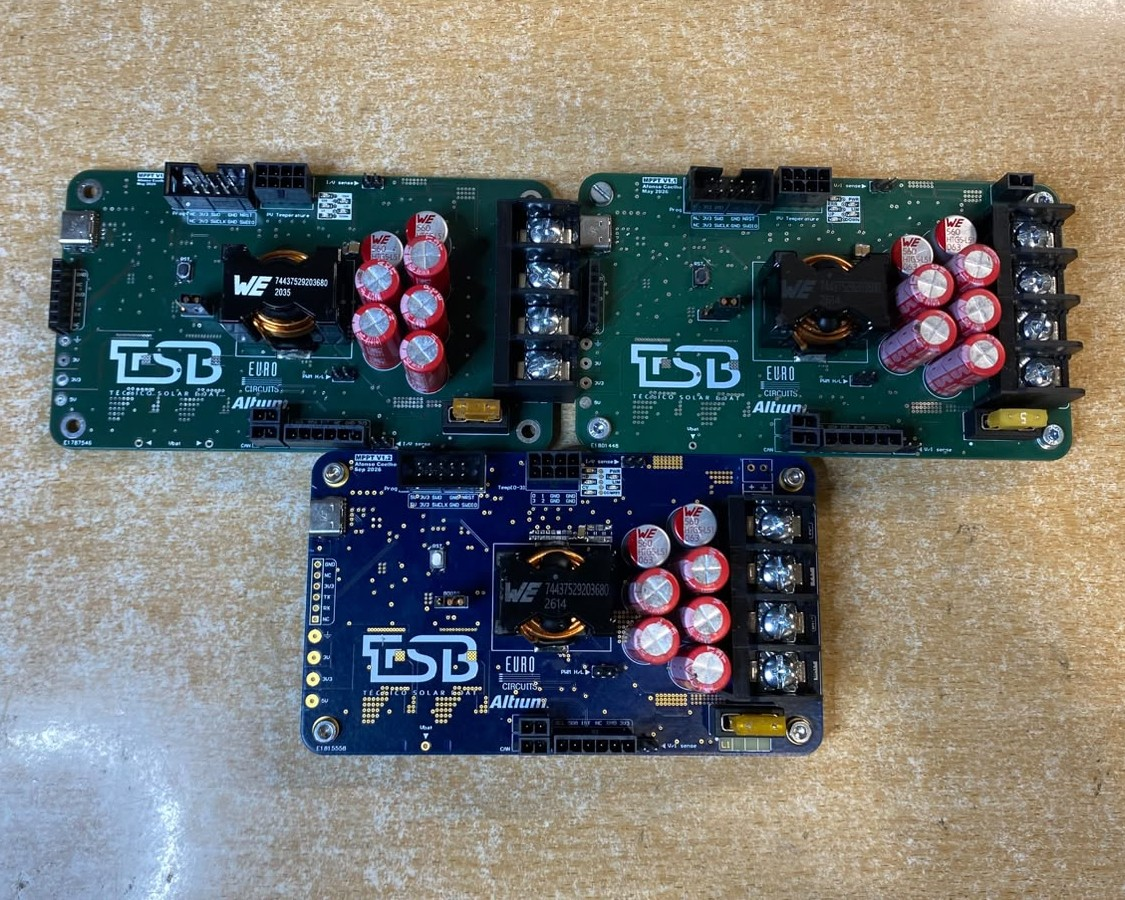
\includegraphics[width=0.99\textwidth]{Images/LAB_res/pcbs.jpeg}
            \caption{Front side.}
        \end{subfigure}
        \hfill
        \begin{subfigure}{0.49\textwidth}
            \centering
            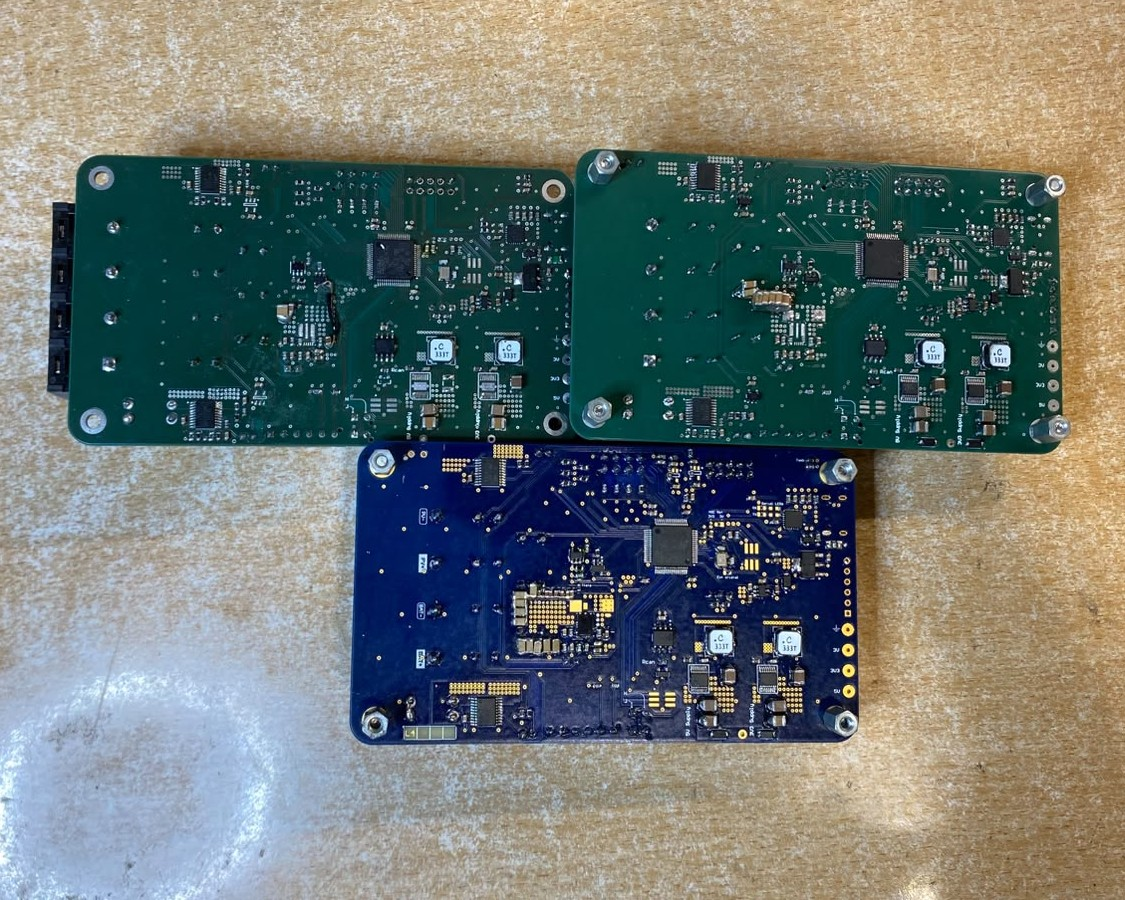
\includegraphics[width=0.99\textwidth]{Images/LAB_res/pcbs_back.jpeg}
            \caption{Back side.}
        \end{subfigure}
        \caption{All prototype versions (V1, V1.1 and V1.2).}
        \label{fig:prototypes}
    \end{figure}

    The \textbf{first prototype (V1)} iteration had several issues identified during the initial testing phase. For instance, an incorrect 3D model caused the main connector to be positioned incorrectly (Figure~\ref{fig:prototypes}).
    Additionally, the flash connector did not provide 5~V, which made testing more difficult. The UART signals connected to the USB-C connector were swapped, and therefore the communication was only possible using an external USB to UART adapter. 

    Although none of these issues were critical for the fundamental operation of the circuit, they made the testing phase more time-consuming and complex. Therefore, a second iteration was designed and manufactured with all issues fixed. 

    Besides the errors found in the first prototype, in the \textbf{second iteration (V1.1)}, two Schottky diodes were placed in parallel with the boost transistors, which, according to the transistor datasheet, should improve the boost converter's efficiency. After some simulations, it was found that this statement does not apply in this case due to the short dead time. Furthermore, during testing of the first iteration, an increase in the inductor temperature was observed. To address the possibility of requiring additional cooling, a connector was added to place a fan if needed. These will also be analyzed in this section.

    Near the end, a \textbf{final version (V1.2)} was made, which includes the extra filter capacitors to filter noise, which will be discussed later. Additionally, the sensors filters were placed near the sensors. Since switching devices generate electromagnetic noise, the filters should be close to the \ac{mcu} pins.  

    Due to time constraints, the majority of the results presented in the following sections were obtained using version V1.1. Whenever results obtained with the latest version are presented, this will be explicitly stated, otherwise, the results refer to version V1.1.


\section{Voltage and current sensor}
    Both current and voltage sensors were tested in the laboratory to validate measurement performance and accuracy. 

    The voltage sensor test was performed by applying a known voltage to the input and measuring MCU readings. 

    The test covered the full voltage range required for the application, from $0$~V to $51$~V. The results demonstrate that the voltage sensors provide accurate measurements, with average absolute errors of $60$~mV for the battery voltage measurement and $112$~mV for the solar panel voltage measurement. The error is different for each sensor because it depends on the actual resistance of the resistors used in the voltage dividers and the \ac{pcb} layout. For each board, the error will be different, but it is expected to be in the same order of magnitude since the tolerance of the resistors is equal.

    These could be improved even further by using resistors with lower tolerance and a lower temperature coefficient, or by increasing the ADC resolution. Another option that does not increase system cost is to subtract the linear error from the results. The magnitude of the error is small, and therefore it does not affect the \ac{mppt} operation, however, for the purpose of this project, the linearization was implemented in firmware to improve the accuracy of the measurements made during the testing phase.

    In Figure~\ref{fig:voltage_sense_error} the error of the voltage readings is represented. Since the error is linear, the trend line is also shown and used to correct the results and improve measurement accuracy. The figure also shows the results after subtracting the linear error, and the error is significantly reduced. The average error was reduced to 28.325~mV and 29.825~mV for the battery and solar panel, respectively. 

    The same test was performed for the current sensors, the average error was 99.93~mA and 8.5~mA for the solar panel and battery, respectively, which is acceptable for this application. Figure~\ref{fig:current_sense_error} shows the current sensor error and indicates that it is linear on the solar panel side and almost null on the battery side. This can be explained by the fact that at low currents, the error is smaller, and probably the shunt resistor value on the solar panel side is more accurate than the shunt resistor on the battery side. However, it is still small and does not affect the \ac{mppt} operation.

    \begin{figure}[!ht] 
        \centering 
        \begin{minipage}{0.49\textwidth}
             \centering
            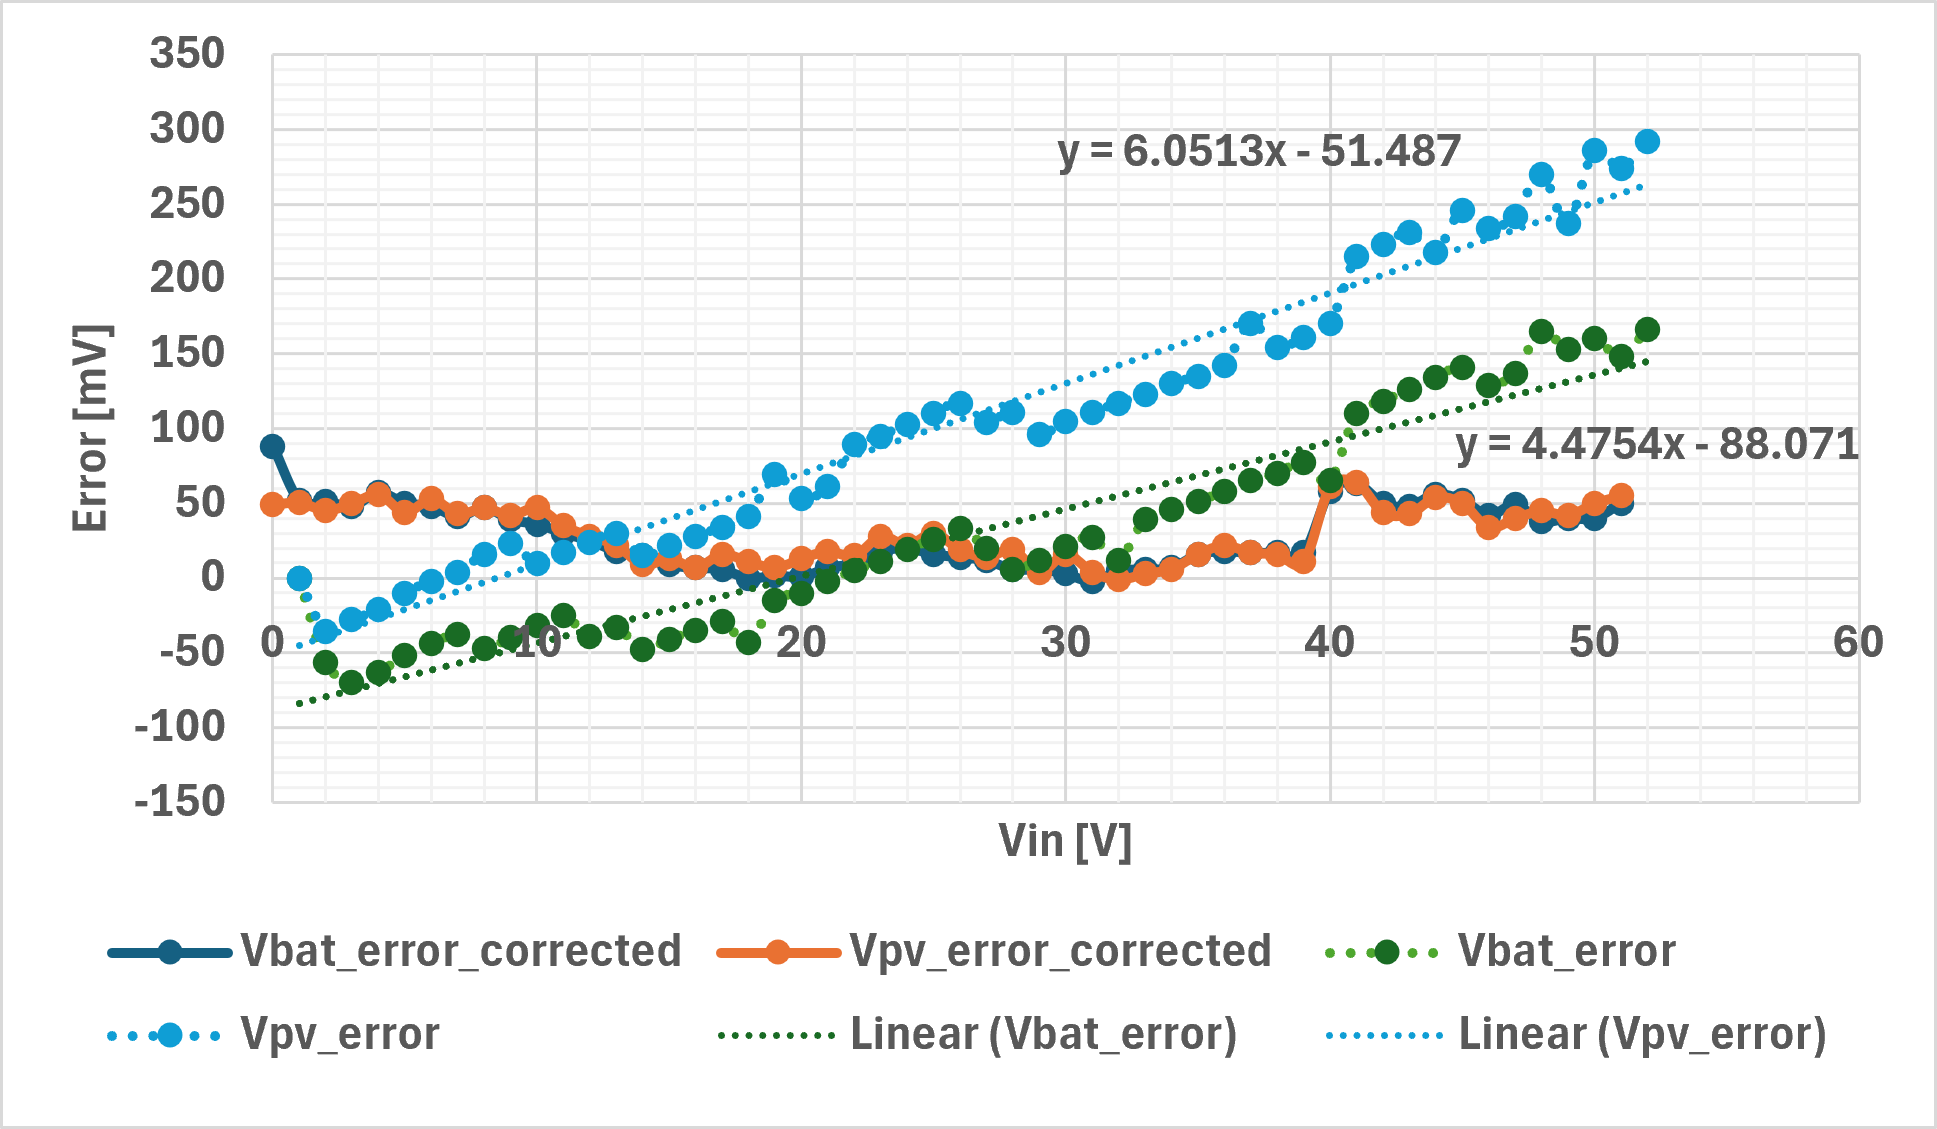
\includegraphics[width=\textwidth]{Images/LAB_res/Voltage_sensor_test.png}
            \caption{Voltage sensor error over voltage.}
            \label{fig:voltage_sense_error}
        \end{minipage} 
        \hfill 
        \begin{minipage}{0.49\textwidth} 
            \centering
            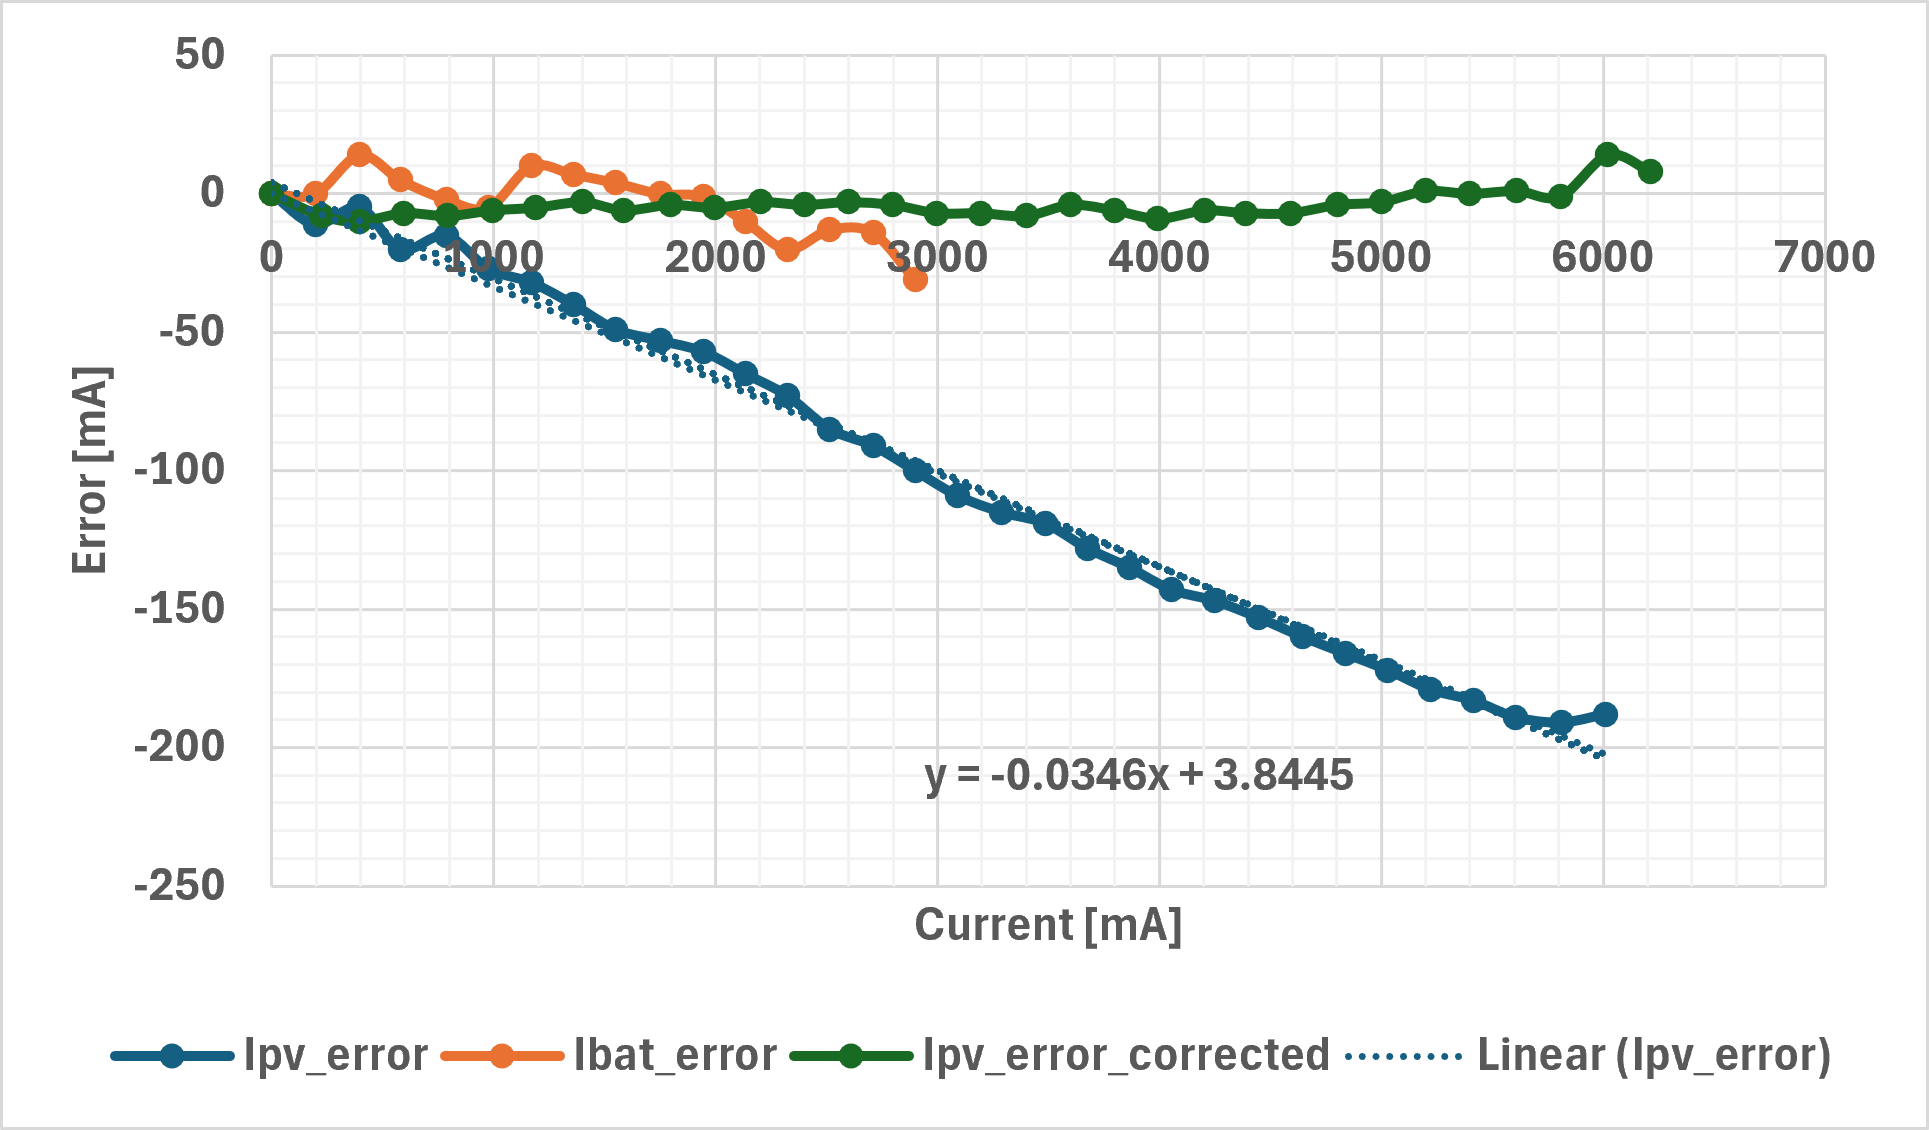
\includegraphics[width=\textwidth]{Images/LAB_res/Current_sensor_test.png}
            \caption{Current sensor error over current.}
            \label{fig:current_sense_error}
        \end{minipage} 
    \end{figure}

    As in the case of the voltage sensor, the subtraction of the linear error would greatly increase the accuracy of the measurements. However, it takes a lot of time to do the measurements and calculate the linearization for each \ac{pcb} which is not realistic for a student prototype project like \ac{tsb}. However, to increase the accuracy of the laboratory results, error correction was implemented for the \ac{pv} side current sensor. The figure also shows the results after subtracting the linear error, and the error is significantly reduced. The average error was reduced to 5.28~mA.

    Another factor affecting the accuracy of the measurements is electrical noise. In prototype version 1.1, the filtering components were placed close to the sensors. In practice, this configuration primarily attenuated noise generated locally by the sensors themselves. However, switching converters are also significant sources of electrical noise, which should be attenuated as close as possible to the ADC/\ac{mcu}. Therefore, the filter placement was modified in version 1.2. The resulting difference in measurement quality is shown in Figure~\ref{fig:sensors noise}, where the measurements were collected at a fixed duty cycle.

    \begin{figure}[!ht]
        \centering
        \begin{subfigure}{0.49\textwidth}
            \centering
            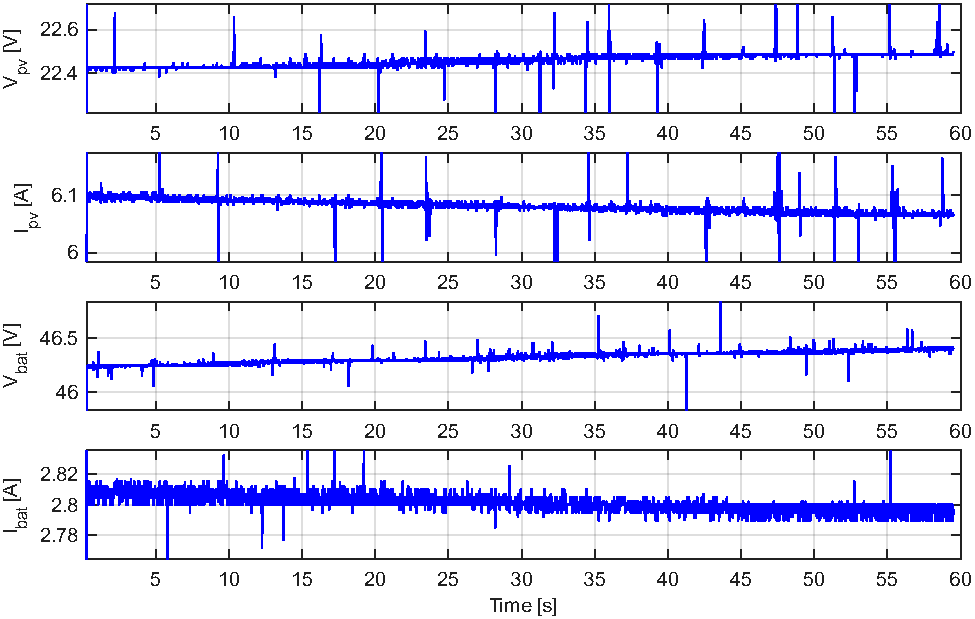
\includegraphics[width=0.99\textwidth]{Images/LAB_res/noise_V1.1.pdf}
            \caption{Version 1.1.}
        \end{subfigure}
        \hfill
        \begin{subfigure}{0.49\textwidth}
            \centering
            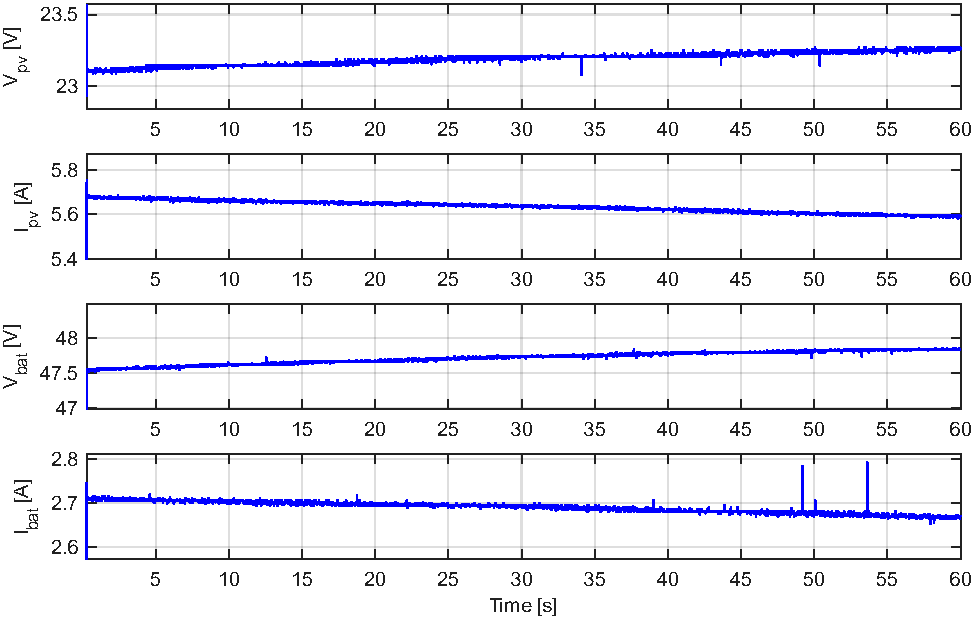
\includegraphics[width=0.99\textwidth]{Images/LAB_res/noise_V1.2_2.pdf}
            \caption{Version 1.2.}
        \end{subfigure}
        \caption{Comparison of sensor readings over a one-minute interval at a fixed duty cycle.}
        \label{fig:sensors noise}
    \end{figure}

    The difference between the two versions is clearly noticeable. In version 1.1, all measurements exhibited significant noise. In contrast, the modified filter configuration in version 1.2 substantially reduced the observed noise to an acceptable level. The battery current measurement represented the worst-case condition, with two distinct spikes occurring during the one minute measurement interval.



\section{Boost}
    The Boost test is essential to identify the efficiency and the correct operation of the synchronous boost converter without the influence of the control system. Additionally, it is essential to confirm the correct dimensioning of the power converter, enabling a comparison with simulations and theoretical calculations.

    The test was performed using a voltage source on the input side and two power resistors on the load side. Both duty cycle and load resistance were varied to obtain the results in all different points of the charging curve.

    All the measurements were performed with a high precision multimeter. The voltage readings were performed as close as possible to the \ac{pcb}, whereas the current readings they have to be performed in line.

    It is important to note that this board uses the battery side to power itself, however, in this test the battery side is not connected to a battery but since the \ac{pv} side is connected to a voltage source, this energy flows to the battery side through the boost converter diodes/body diodes and therefore powers the control system.
        
    \subsection{Switching noise}
        During the initial experimental tests, significant electrical noise was observed in all measured signals. The resulting current fluctuations repeatedly exceeded the configured \ac{oc} protection thresholds, causing the converter to enter an undesirable protection cycle. Firmware modifications were therefore implemented, including increasing the ADC sampling time and the number of samples used for each measurement, with the final value obtained by averaging the samples. The fault-handling logic was also modified to introduce a $5~\mathrm{s}$ delay before verifying whether the fault condition had been cleared. Although these changes improved measurement stability, they did not eliminate the excessive noise.

        The input current was observed to oscillate significantly during \ac{oc} events, with values ranging approximately from $4~\mathrm{A}$ to $12~\mathrm{A}$. Initially, the laboratory power supply was considered a possible cause, as it was operating close to its current limit. However, comparison with the reference evaluation board revealed a significant difference in the output decoupling network. The initial prototype used only a single $1~\mu\mathrm{F}$ ceramic capacitor, whereas the reference board employed ten $1~\mu\mathrm{F}$ capacitors in parallel.

        The converter was therefore characterized before and after increasing the output decoupling capacitance. Figure~\ref{fig:ruido inicial} shows the initial measurements. Nine additional $1~\mu\mathrm{F}$ ceramic capacitors were then connected in parallel with the existing capacitor, reproducing the total capacitance of the reference board. This modification resulted in a substantial reduction in the observed switching noise, as shown in Figure~\ref{fig:ruido final}.

        Additional high-frequency decoupling was subsequently implemented by adding six $100~\mathrm{nF}$ ceramic capacitors, replacing the additional $220~\mathrm{nF}$ capacitors used in the reference design due to component availability. The resulting waveforms are shown in Figure~\ref{fig:ruido final 2}. A further reduction in current noise was observed, although the measured input voltage noise increased slightly. This difference is likely related to measurement inaccuracy.

        The influence of the Schottky diodes placed in parallel with the boost transistors was also evaluated. The resulting waveforms are shown in Figure~\ref{fig:ruido final 3}. The addition of the diodes did not significantly affect the measured noise, although a slight increase in input voltage noise was observed. The decision was to not include them since neither the noise nor the efficiency improved significantly, and they increased the cost of the prototype.

        The approximate noise amplitudes measured for the different hardware configurations are summarized in Table~\ref{tab:noise_comparison}. The addition of the nine $1~\mu\mathrm{F}$ capacitors produced the most significant improvement, particularly in the input current and voltage measurements. The subsequent addition of the $100~\mathrm{nF}$ capacitors provided a further reduction in current noise.

        Overall, the experimental results indicate that insufficient output decoupling was the primary contributor to the excessive switching noise observed in the initial prototype. Increasing the local output capacitance substantially reduced the noise and improved the stability of the converter. The noise amplitudes presented in Table~\ref{tab:noise_comparison} should, however, be considered approximate, as a more controlled measurement procedure with an appropriate oscilloscope trigger would be required to accurately quantify the peak noise amplitudes.


        \begin{table}[!ht]
            \centering
            \caption{Approximate noise amplitudes measured for the three hardware configurations.}
            \label{tab:noise_comparison}
            \begin{tabular}{|l|cccc|}
                \hline
                Quantity &
                Original &
                +9 $\times$ $1~\mu\mathrm{F}$ &
                +9 $\times$ $1~\mu\mathrm{F}$ +6 $\times$ $100~\mathrm{nF}$ &
                All + schottky diode\\
                \hline
                $I_{in}$  & 1.8~A   & 640~mA & 292~mA & 140~mA \\
                $I_{out}$ & 0.8~A   & 300~mA & 220~mA & 272~mA \\
                $V_{in}$  & 2.0~V   & 350~mV & 380~mV & 490~mV \\
                $V_{out}$ & 8.0~V   & 2.3~V  & 2.2~V  & 1.440~V \\
                \hline 
            \end{tabular}
        \end{table}

        \begin{figure}[!ht] 
            \centering 
            \begin{minipage}{0.49\textwidth}
               \centering 
                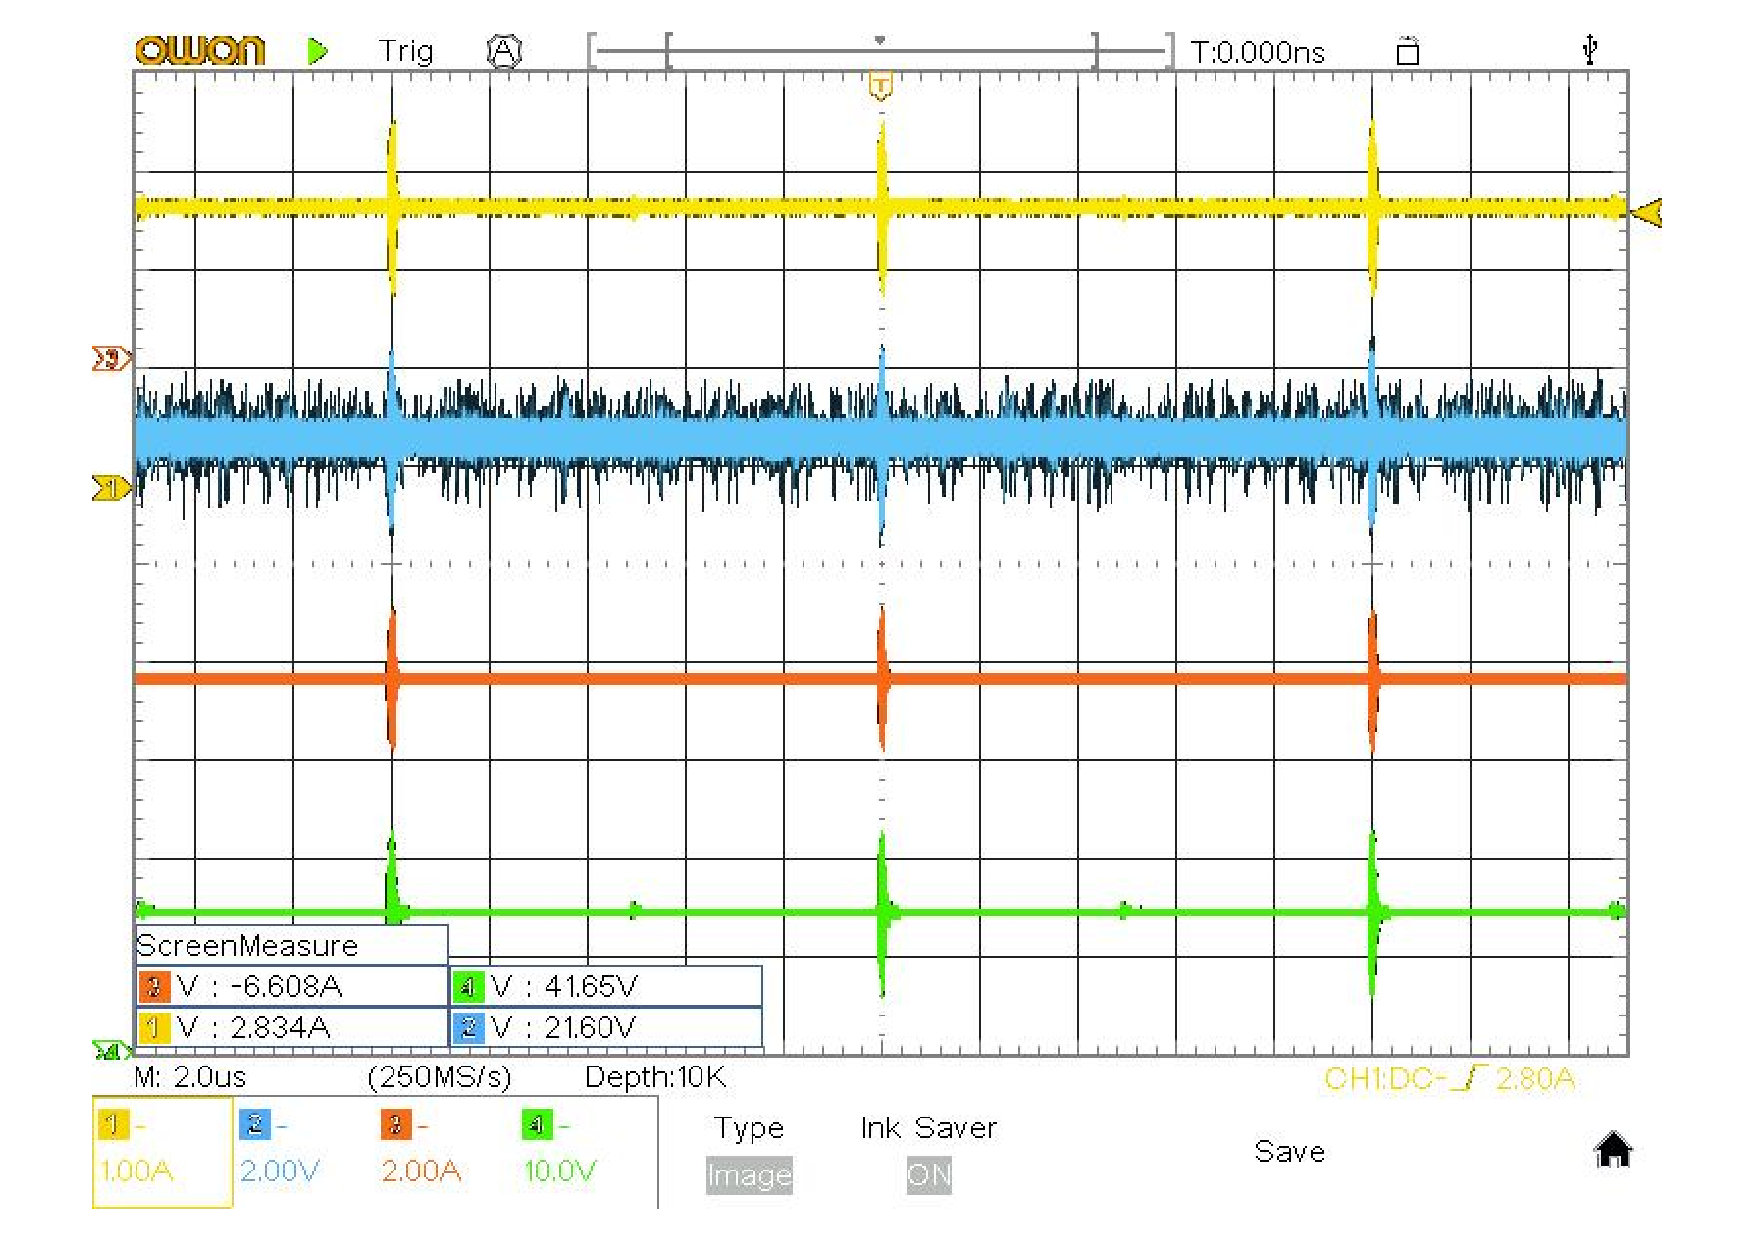
\includegraphics[width=\linewidth]{Images/LAB_res/case2-1.pdf} 
                \caption{Measured waveforms before adding the additional ceramic capacitors.} 
                \label{fig:ruido inicial}
            \end{minipage} 
            \hfill 
            \begin{minipage}{0.49\textwidth} 
                \centering 
                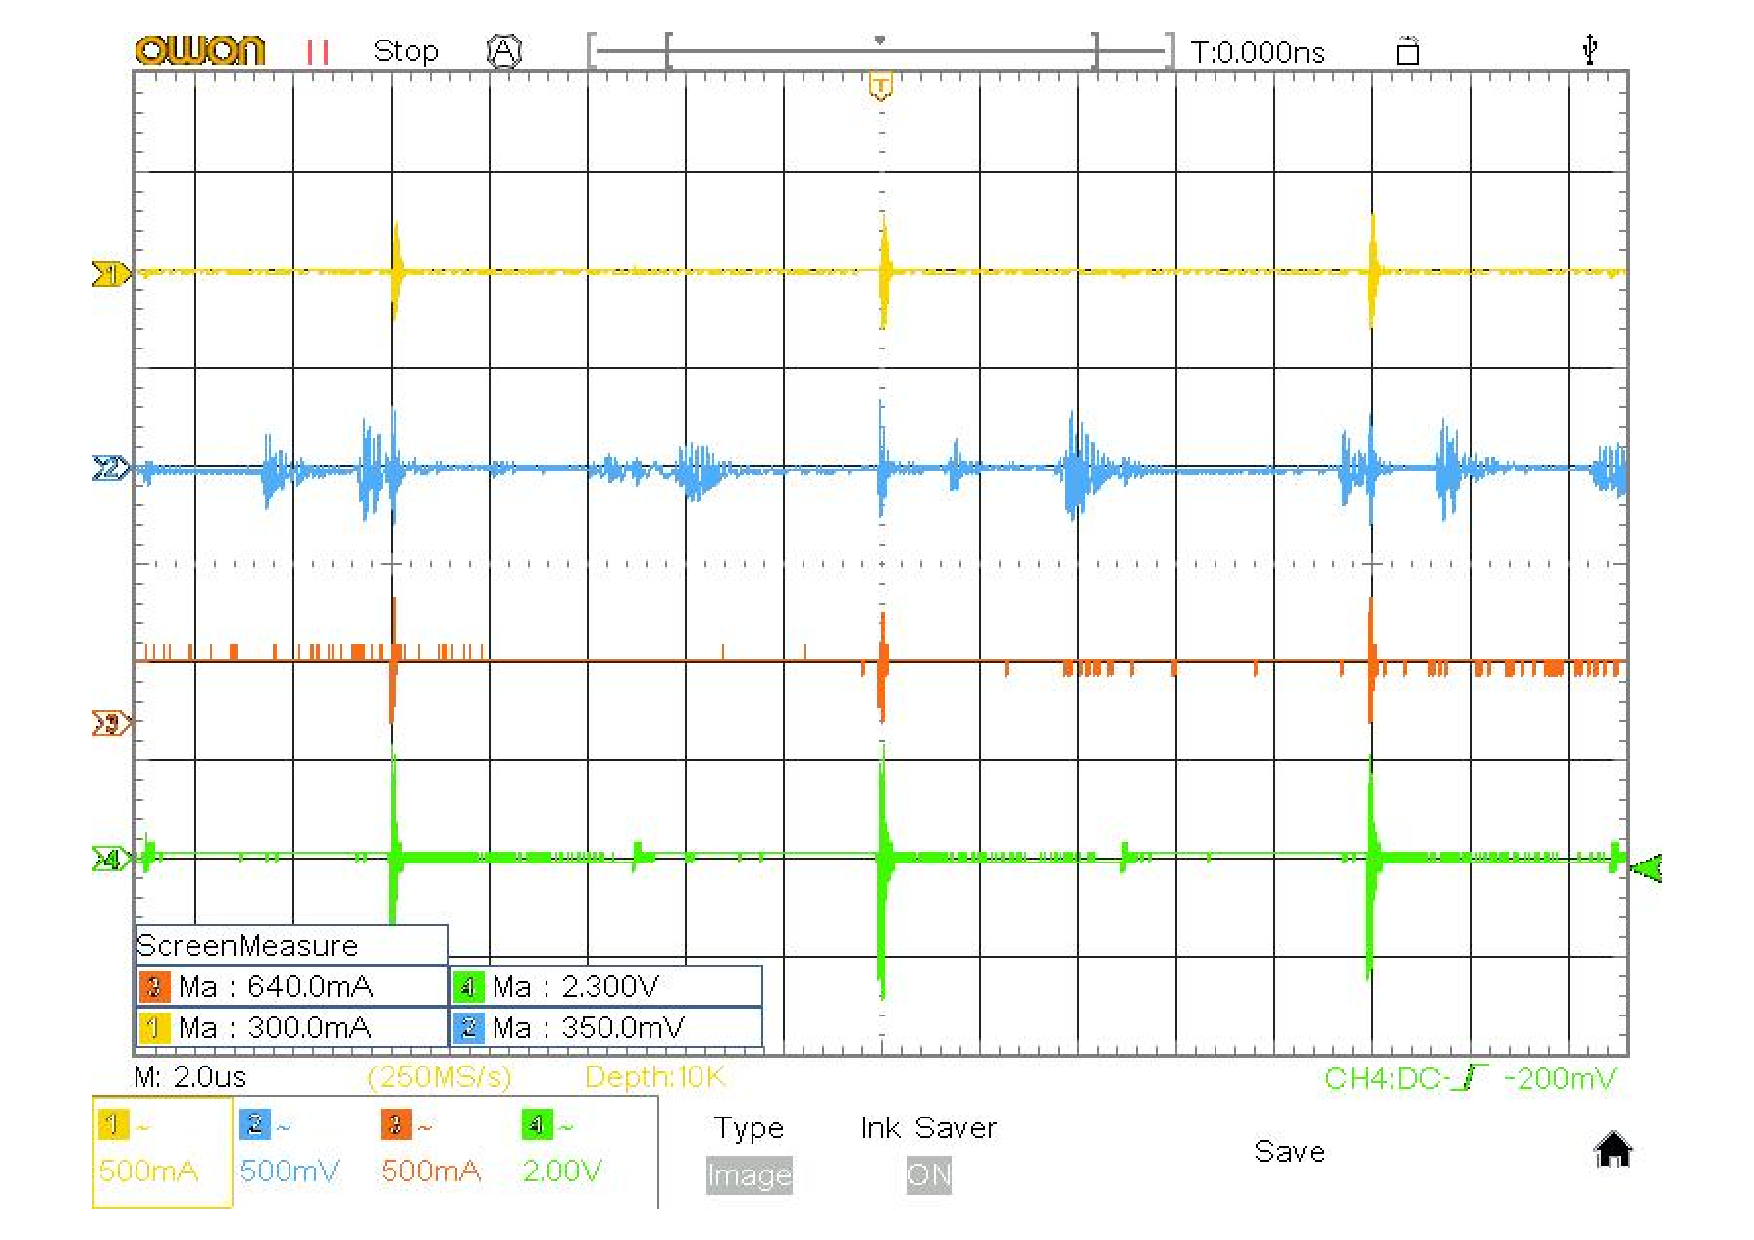
\includegraphics[width=\linewidth]{Images/LAB_res/case2-2.pdf}
                \caption{Measured waveforms after adding nine additional $1~\mu\mathrm{F}$ ceramic capacitors.} 
                \label{fig:ruido final} 
            \end{minipage} 
        \end{figure}

        \begin{figure}[!ht] 
            \centering 
            \begin{minipage}{0.49\textwidth}
                \centering 
                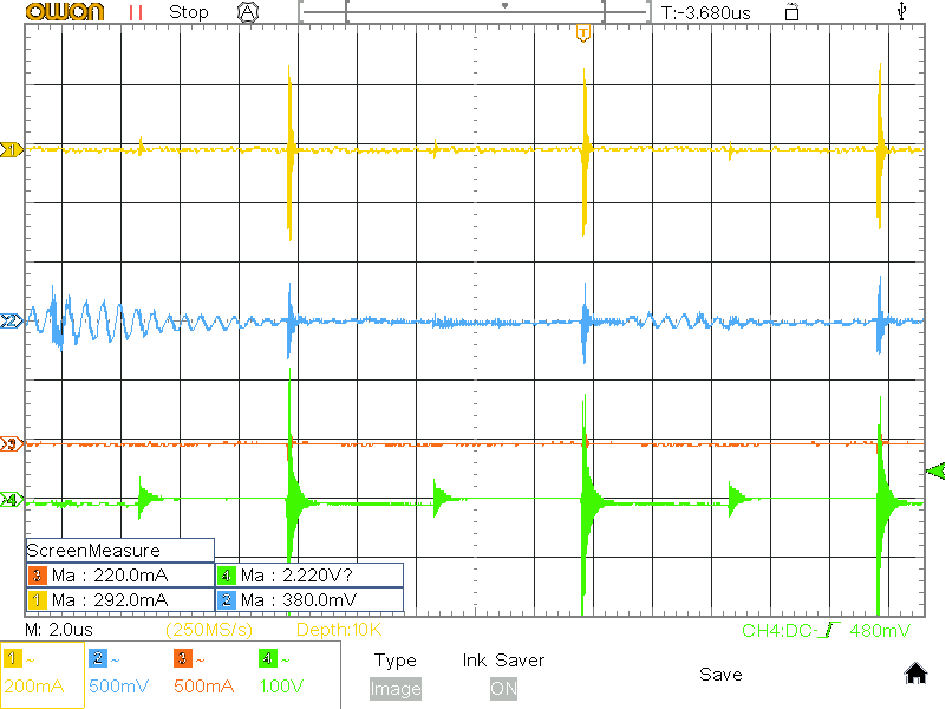
\includegraphics[width=0.9\linewidth]{Images/LAB_res/case2-3.pdf} 
                \caption{Measured waveforms after adding six additional $100~\mathrm{nF}$ ceramic capacitors.} 
                \label{fig:ruido final 2} 
            \end{minipage} 
            \hfill 
            \begin{minipage}{0.49\textwidth} 
                \centering 
                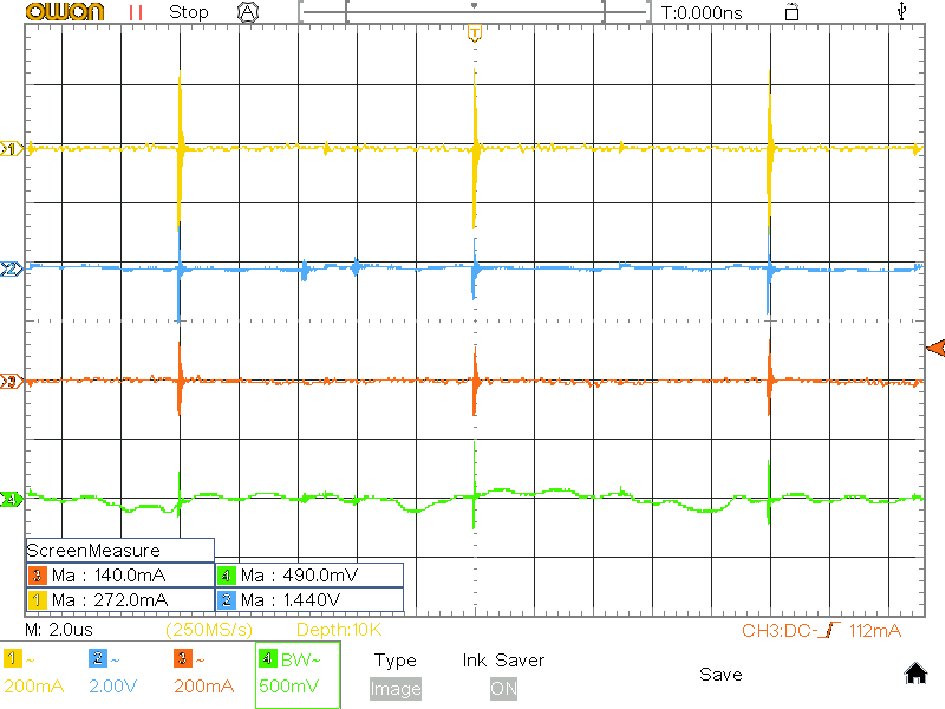
\includegraphics[width=0.9\linewidth]{Images/LAB_res/noise-w_diode.pdf} 
                \caption{Measured waveforms after adding two Schottky diodes (channels 4 and 2 are swapped compared to the other figures).} 
                \label{fig:ruido final 3} 
            \end{minipage} 
        \end{figure}

        Since the precision of the previous measurement is insufficient to enable a meaningful comparison with other devices, an additional test was performed to characterize the conducted noise spectrum of the prototype.

        The test procedure was based on the CISPR 25:2021 standard, which specifies methods for measuring radio disturbances generated by electrical and electronic components intended for use in vehicles. This standard was selected because one of the main concerns associated with electromagnetic noise in the prototype is the potential interference with communication systems used in the vessel, such as CAN and VHF communication systems. CISPR 25 defines measurement procedures and limits for conducted disturbances on power supply lines. The limits are divided into five EMC classes, with Class 5 representing the most stringent limits. The limits considered in this analysis are presented in Table~\ref{tab:cispr25_limits}.

        \begin{table}[htbp]
            \centering
            \caption{CISPR 25 EMI noise limitations.}
            \label{tab:cispr25_limits}
            \begin{tabular}{|c|cc|cc|cc|cc|cc|}
                \hline
                \multirow{2}{*}{\textbf{EMC Class}} &
                \multicolumn{10}{c|}{\textbf{Magnitude (dB$\mu$V)}} \\
                \cline{2-11}
                & \multicolumn{2}{c|}{0.15--0.3~MHz} &
                \multicolumn{2}{c|}{0.53--2~MHz} &
                \multicolumn{2}{c|}{5.9--6.2~MHz} &
                \multicolumn{2}{c|}{30--54~MHz} &
                \multicolumn{2}{c|}{68--108~MHz} \\
                & Peak & Average & Peak & Average & Peak & Average &
                Peak & Average & Peak & Average \\
                \hline
                1 & 113 & 100 & 95 & 82 & 77 & 64 & 77 & 64 & 61 & 48 \\
                2 & 103 & 90  & 87 & 74 & 71 & 58 & 71 & 58 & 55 & 42 \\
                3 & 93  & 80  & 79 & 66 & 65 & 52 & 65 & 52 & 49 & 36 \\
                4 & 83  & 70  & 71 & 58 & 59 & 46 & 59 & 46 & 43 & 30 \\
                5 & 73  & 60  & 63 & 50 & 53 & 40 & 53 & 40 & 37 & 24 \\
                \hline
            \end{tabular}
        \end{table}

        The prescribed test procedure was not fully reproduced due to equipment limitations. In particular, a Line Impedance Stabilization Network (LISN), which is normally used to provide a defined impedance and isolate the measurement from disturbances originating from the external power supply, was not available. Furthermore, the measurements were not performed inside a shielded enclosure, such as a Faraday cage, and were therefore potentially affected by external electromagnetic disturbances. Consequently, the results should not be interpreted as a formal CISPR 25 compliance test. Nevertheless, the measurements provide a useful indicative characterization of the conducted noise generated by the prototype. Since the absence of a LISN and shielding can introduce additional external disturbances, measured values below the specified limits provide an indication that the prototype's conducted emissions are unlikely to exceed those limits under the tested conditions.

        The test setup consisted of a DC power supply set to 22~V and a resistive load of 10~$\Omega$. The prototype operated with a duty cycle of 52.5\%. The resulting noise spectrum is presented in Figure~\ref{fig:noise_w_load}. The measurement was subsequently repeated with no external load while maintaining a fixed output voltage of 50.4~V. The corresponding spectrum is presented in Figure~\ref{fig:noise_w_no_load}.

        \begin{figure}[!ht]
        \centering
        \begin{minipage}{0.49\textwidth}
        \centering
        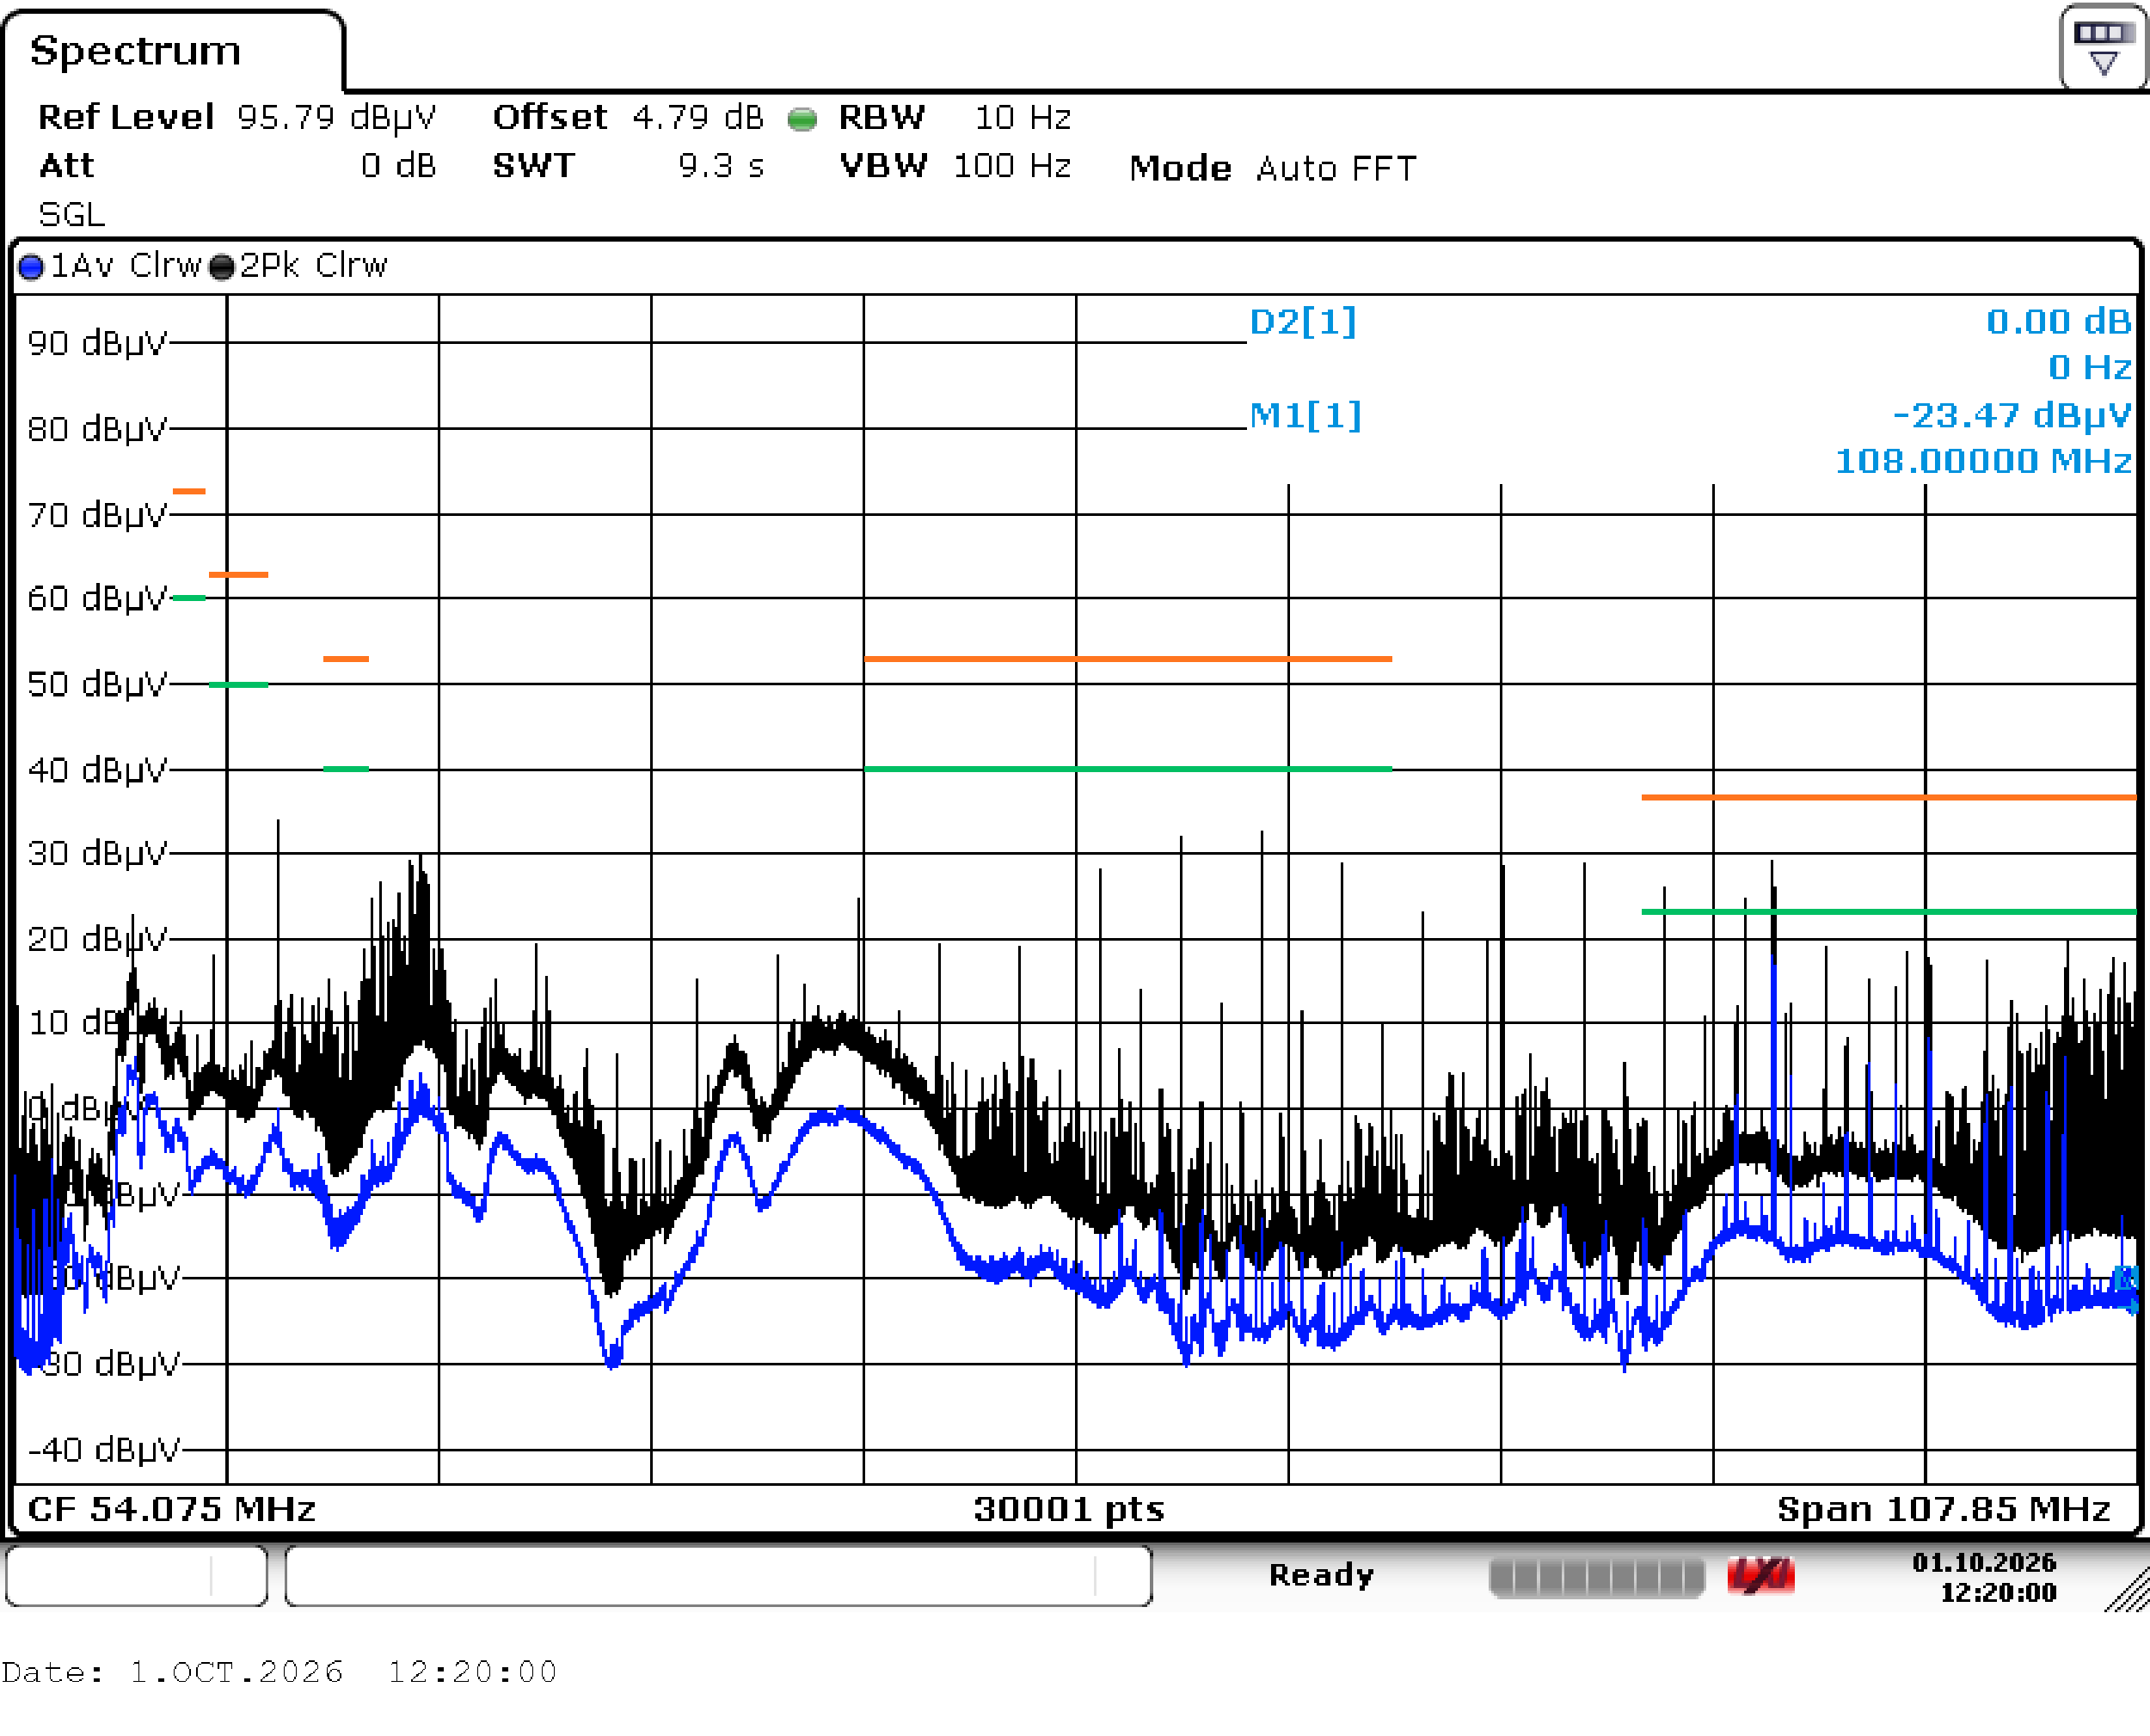
\includegraphics[width=\linewidth]{Images/LAB_res/noise_w_load.pdf}
        \caption{Noise spectrum with a 10~$\Omega$ load.}
        \label{fig:noise_w_load}
        \end{minipage}
        \hfill
        \begin{minipage}{0.49\textwidth}
        \centering
        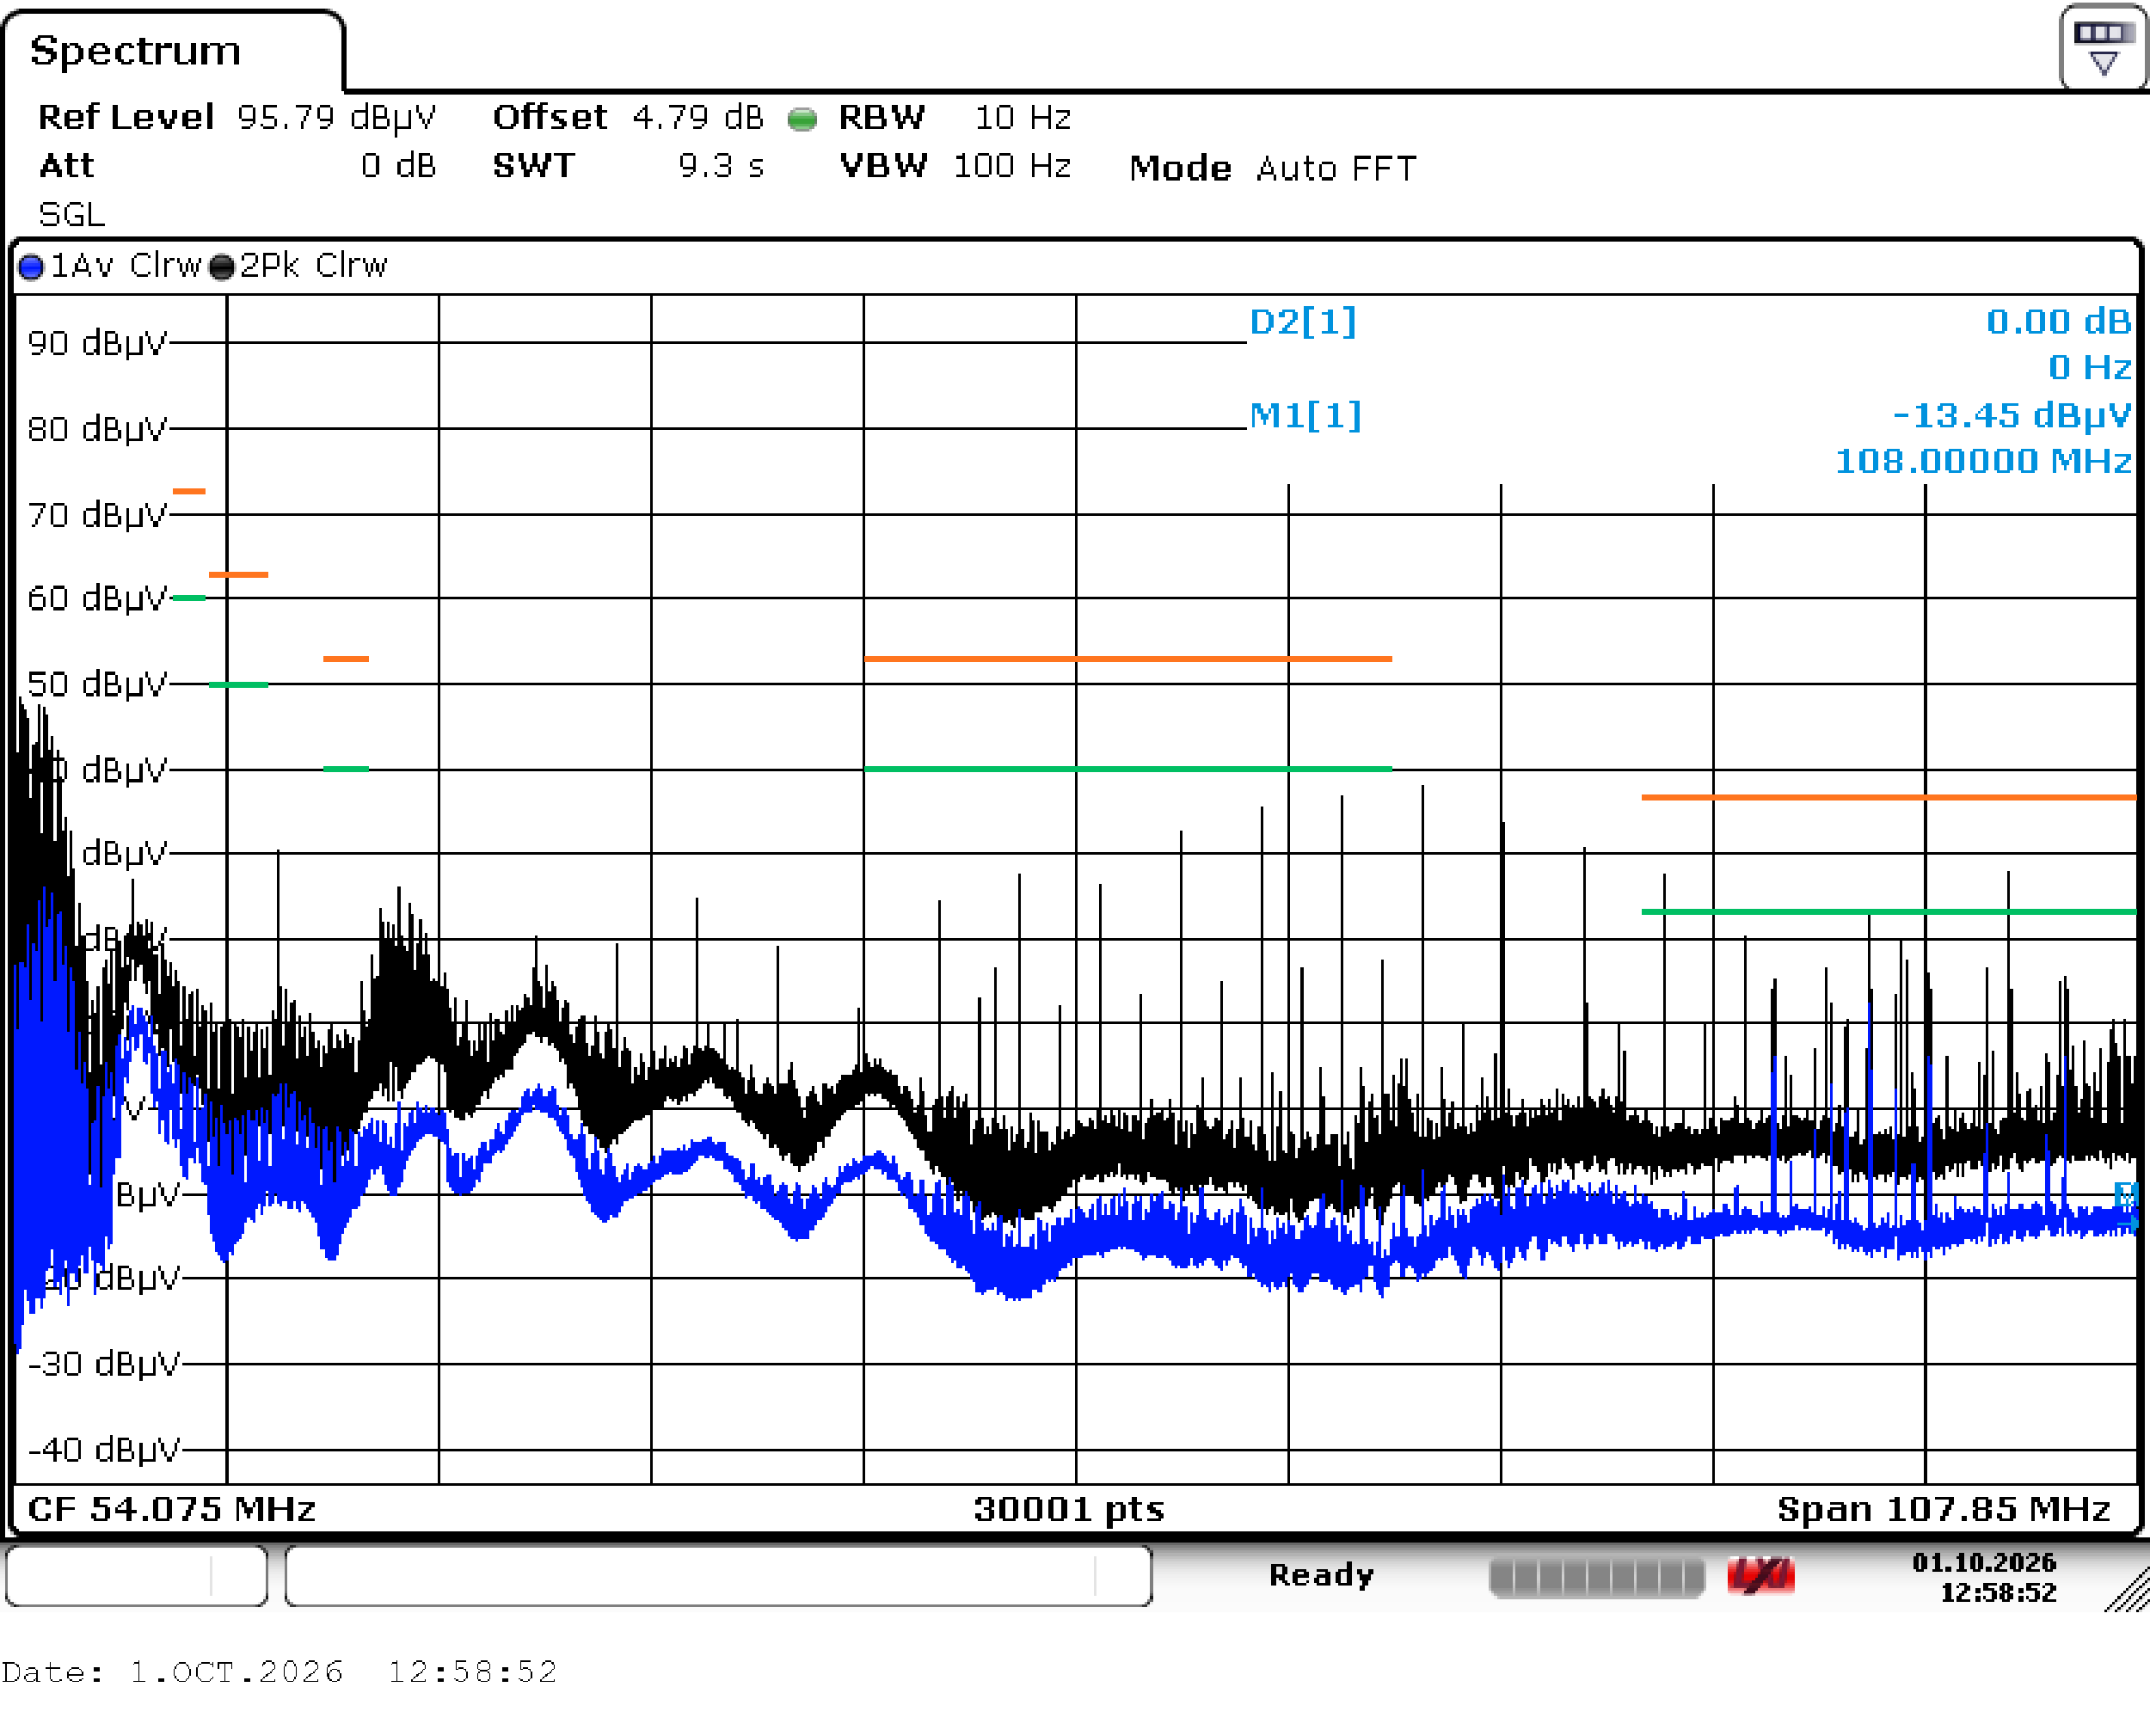
\includegraphics[width=\linewidth]{Images/LAB_res/noise_w_no_load.pdf}
        \caption{Noise spectrum with no external load.}
        \label{fig:noise_w_no_load}
        \end{minipage}
        \end{figure}

        Both measurements show that the measured noise remains below the Class 5 limits over the frequency ranges considered. Therefore, despite the limitations of the experimental setup, the results indicate a low level of conducted emissions from the prototype when compared with the most stringent limits considered in CISPR 25.

        The average noise level is higher in the no-load condition. This behavior can be associated with the different operating conditions of the converter at light load. In particular, reduced load current can lead to changes in the switching current waveform and operating regime of the converter, potentially increasing the relative contribution of high frequency components to the measured spectrum.         
        

    \subsection{Efficiency}
        The efficiency of the \ac{mppt} charger is one of the most important parameters to measure because it directly affects the power effectively extracted from the solar panel and delivered to the battery. As in simulations, the efficiency was measured for each point of the charging curve. All the measurements were taken with the multimeter and the results are presented in Table~\ref{tab:efficiency_results}.

        \begin{table}[!ht]
            \centering
            \caption{Efficiency measurements for the different test cases.}
            \label{tab:efficiency_results}
            \begin{tabular}{|l|ccc|cc|}
                \hline
                & \multicolumn{3}{c|}{Multimeter} 
                & - OC power 
                & - OC+Transistors power \\
                \hline
                Case & Power in & Power out & Efficiency 
                & Efficiency & Efficiency \\
                \hline
                Case 1 & 127.444 & 123.413 & 96.84\% & 97.23\% & 97.64\% \\
                Case 2 & 129.108 & 124.685 & 96.57\% & 96.96\% & 97.36\% \\
                Case 3 & 127.523 & 123.232 & 96.64\% & 97.02\% & 97.43\% \\
                Case 4 & 73.1277 & 70.818 & 96.84\% & 97.52\% & 98.24\% \\
                \hline
                OC & 0.5103 & 0 & -- & -- & -- \\
                OC+Transistors & 1.04279 & 0 & -- & -- & -- \\
                \hline
            \end{tabular}
        \end{table}

        The measured efficiency exceeds 96\% across all test cases, which is higher than the goal (90\%). This efficiency accounts for all converter losses, including the measurement and control systems. Compared with the power loss estimate in section~\ref{subsubsec:loss_estimation}, the efficiency is about 2\% lower than expected. This difference can be explained by the fact that the components used can have slightly different characteristics. Also, the estimation did not account for losses caused by the parasitic elements of the \ac{pcb}.

        The \ac{pcb} was also tested in open circuit with and without driving the transistors. The results show the losses of the circuit without the boost converter. Around 0.5~W of losses are caused only by the measurement and control system. When the transistors are driven without any load, the converter losses are negligible because the current is too low. So the measured losses are approximately equal to the driving circuit + the measurement and control system. Based on these values, Table~\ref{tab:efficiency_results} also presents an estimate of the efficiency without the measurement and control system, and another without the driving circuit. The converter efficiency is around 97\% to 98\% for all test cases, which is close to the simulation measurements. From another perspective, this shows how significant the losses are in the rest of the circuit.         

    \subsection{Temperature rise}
        The temperature of each element was measured before each test and after 10~min. All test show similar result, a temperature rise of up to $10~^\circ\mathrm{C}$. The inductor is the main heat element, reaching $43~^\circ\mathrm{C}$, the capacitors also reach around $40~^\circ\mathrm{C}$ however, they are placed side by side with the inductor which heats the capacitors. As expected, the transistors do not overheat. The maximum temperature measured was $40~^\circ\mathrm{C}$. 

        The results are consistent with the expected behavior. In Section~\ref{subsubsec:loss_estimation}, it was concluded that the inductor exhibits the highest losses, followed by the transistors and the capacitors. Since the temperature rise is directly related to the power dissipated by each component, a similar trend was expected in the thermal measurements. The results confirm this expectation, with the inductor exhibiting the highest temperature.

        Thermal images of the circuit were also obtained, as shown in Figures~\ref{fig:thermal_front} and \ref{fig:thermal_back}, allowing identification of the areas with the highest temperatures. However, image quality is limited, and a vertical offset is visible between the thermal and visible images. Furthermore, the vertical lines present in the thermal images are measurement artifacts caused by the thermal imaging device and do not represent actual temperature variations.

        Despite these limitations, the results indicate that the inductor reaches the highest temperature, with a noticeable spread of heat to the surrounding area. The capacitors also dissipate some heat, though to a lower extent than the inductor. On the rear side of the PCB, only the transistors show a significant temperature increase.


        \begin{figure}[!ht] 
            \centering 
            \begin{minipage}{0.49\textwidth}
                \centering 
                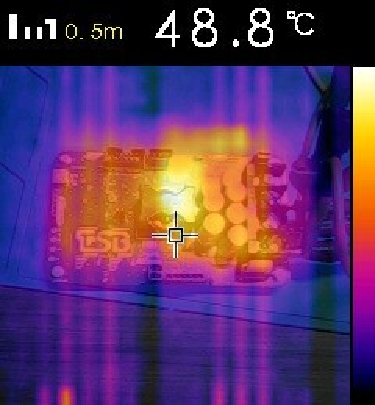
\includegraphics[width=0.7\linewidth]{Images/LAB_res/IMG00029.pdf} 
                \caption{Front side thermal image.} 
                \label{fig:thermal_front} 
            \end{minipage} 
            \hfill 
            \begin{minipage}{0.49\textwidth} 
                \centering 
                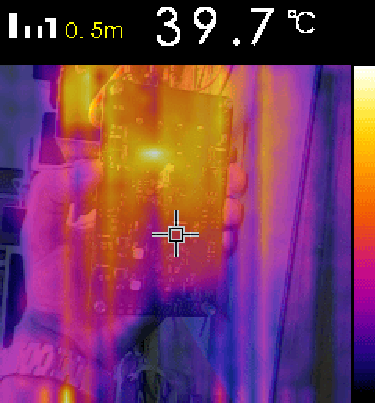
\includegraphics[width=0.7\linewidth]{Images/LAB_res/IMG00030.pdf} 
                \caption{Back side thermal image.} 
                \label{fig:thermal_back} 
            \end{minipage} 
        \end{figure}

        To confirm that the temperature does not rise to a concerning level, a test of 3~h was performed with the converter operating at Case 3. Figure~\ref{fig:3h_temp_test} shows the temperature evolution over the 3~h for the inductor, capacitors, transistors and the ambient temperature. These results were acquired using the thermistors placed on the board, which measure the ambient temperature and the transistors' temperature. The other measurements were acquired using additional external thermistors that can be read by the board using the connector placed for thermistors. 

        The measured values were confirmed using an infrared thermometer which show insignificant difference in temperature, confirming the quality of the measurements.
        
        From Figure~\ref{fig:3h_temp_test}, it can be concluded that after 40~min at maximum power, all the temperatures stop rising. Some oscillations were measured during the experiment because the ambient temperature also oscillated. As seen earlier, the inductor is the element that heats the most, followed by the transistor and capacitors. After 3~h, none of the elements reached a concerning temperature.

        This test concludes that no cooling is needed. At least under the same test conditions. To confirm this statement, the board was placed inside a cardboard box since \ac{tsb} usually places boards inside closed boxes. If the components inside the box need cooling, a fan or water cooling needs to be added.

        Figure~\ref{fig:3h_temp_test_close_box} represents the described test. With no airflow, the ambient temperature reading is more stable, and so are the others. As in the previous test, after 60~min the temperatures remained approximately constant and the maximum temperature was $51.6~^\circ\mathrm{C}$. Since none of the temperatures show concerning values, it is safe to conclude that no additional cooling is needed

        \begin{figure}[!ht] 
            \centering 
            \begin{minipage}{0.49\textwidth}
                 \centering 
                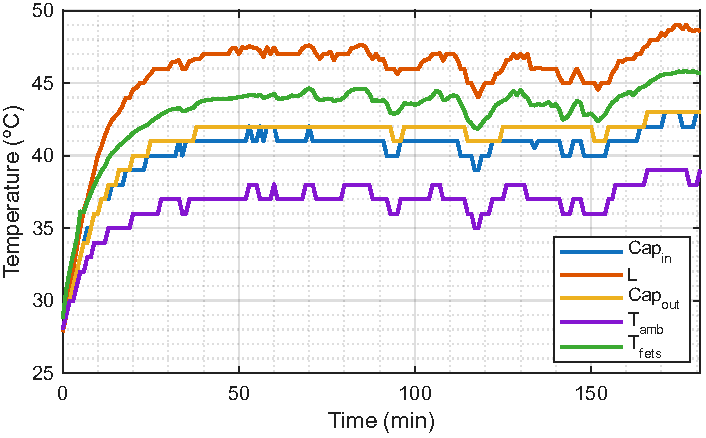
\includegraphics[width=\linewidth]{Images/LAB_res/Temperatures vs time.pdf} 
                \caption{Temperature evolution during 3~h at charging case 3.} 
                \label{fig:3h_temp_test} 
            \end{minipage} 
            \hfill 
            \begin{minipage}{0.49\textwidth} 
                \centering 
            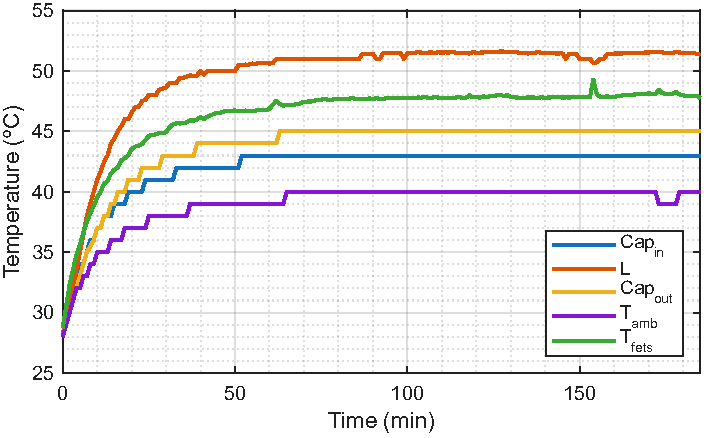
\includegraphics[width=\linewidth]{Images/LAB_res/Temperatures_vs_time_close box.pdf} 
            \caption{Temperature evolution during 3~h at charging case 3 in a closed box.} 
            \label{fig:3h_temp_test_close_box} 
            \end{minipage} 
        \end{figure}


\section{MPPT}
    In this section, the charging state machine is tested, as well as the \ac{mppt} algorithm, to ensure the functionality of the prototype.

    In the following tests, a laboratory setup was used, where a power supply (the SM 1500-CP-30) was used with an internal function that can simulate the behavior of a solar panel. This function was configured as a 35 cells solar panel at $25~^\circ\mathrm{C}$ and variable irradiance controlled by sending TCP messages. 

    The load was the battery from \ac{sr03}, which is described in section~\ref{sec:battery}.

    This setup ensures a controlled environment where the solar panel operates at specified temperature and irradiance, increasing the number of controlled variables. Because the user sets the environmental conditions, this setup can be easily replicated for future comparisons, increasing the scientific value of the tests.

    \subsection{State machine}
        First, the state machine was tested. Figure~\ref{fig:state machine} illustrates the evolution of the different states over time. The state machine responded as expected when both the source and load were disconnected. When both the source and load were connected, the \ac{peo}/\ac{mppt} state was activated. After a few seconds, the irradiance level of the power supply, which was used to emulate a solar panel, was increased, resulting in an increase in the output current. For this test, the \ac{cc} current limit was set to $2~\mathrm{A}$. Consequently, once the output current reached this limit, the state machine transitioned to the \ac{cc} state.

        \begin{figure}[!ht] 
            \centering 
            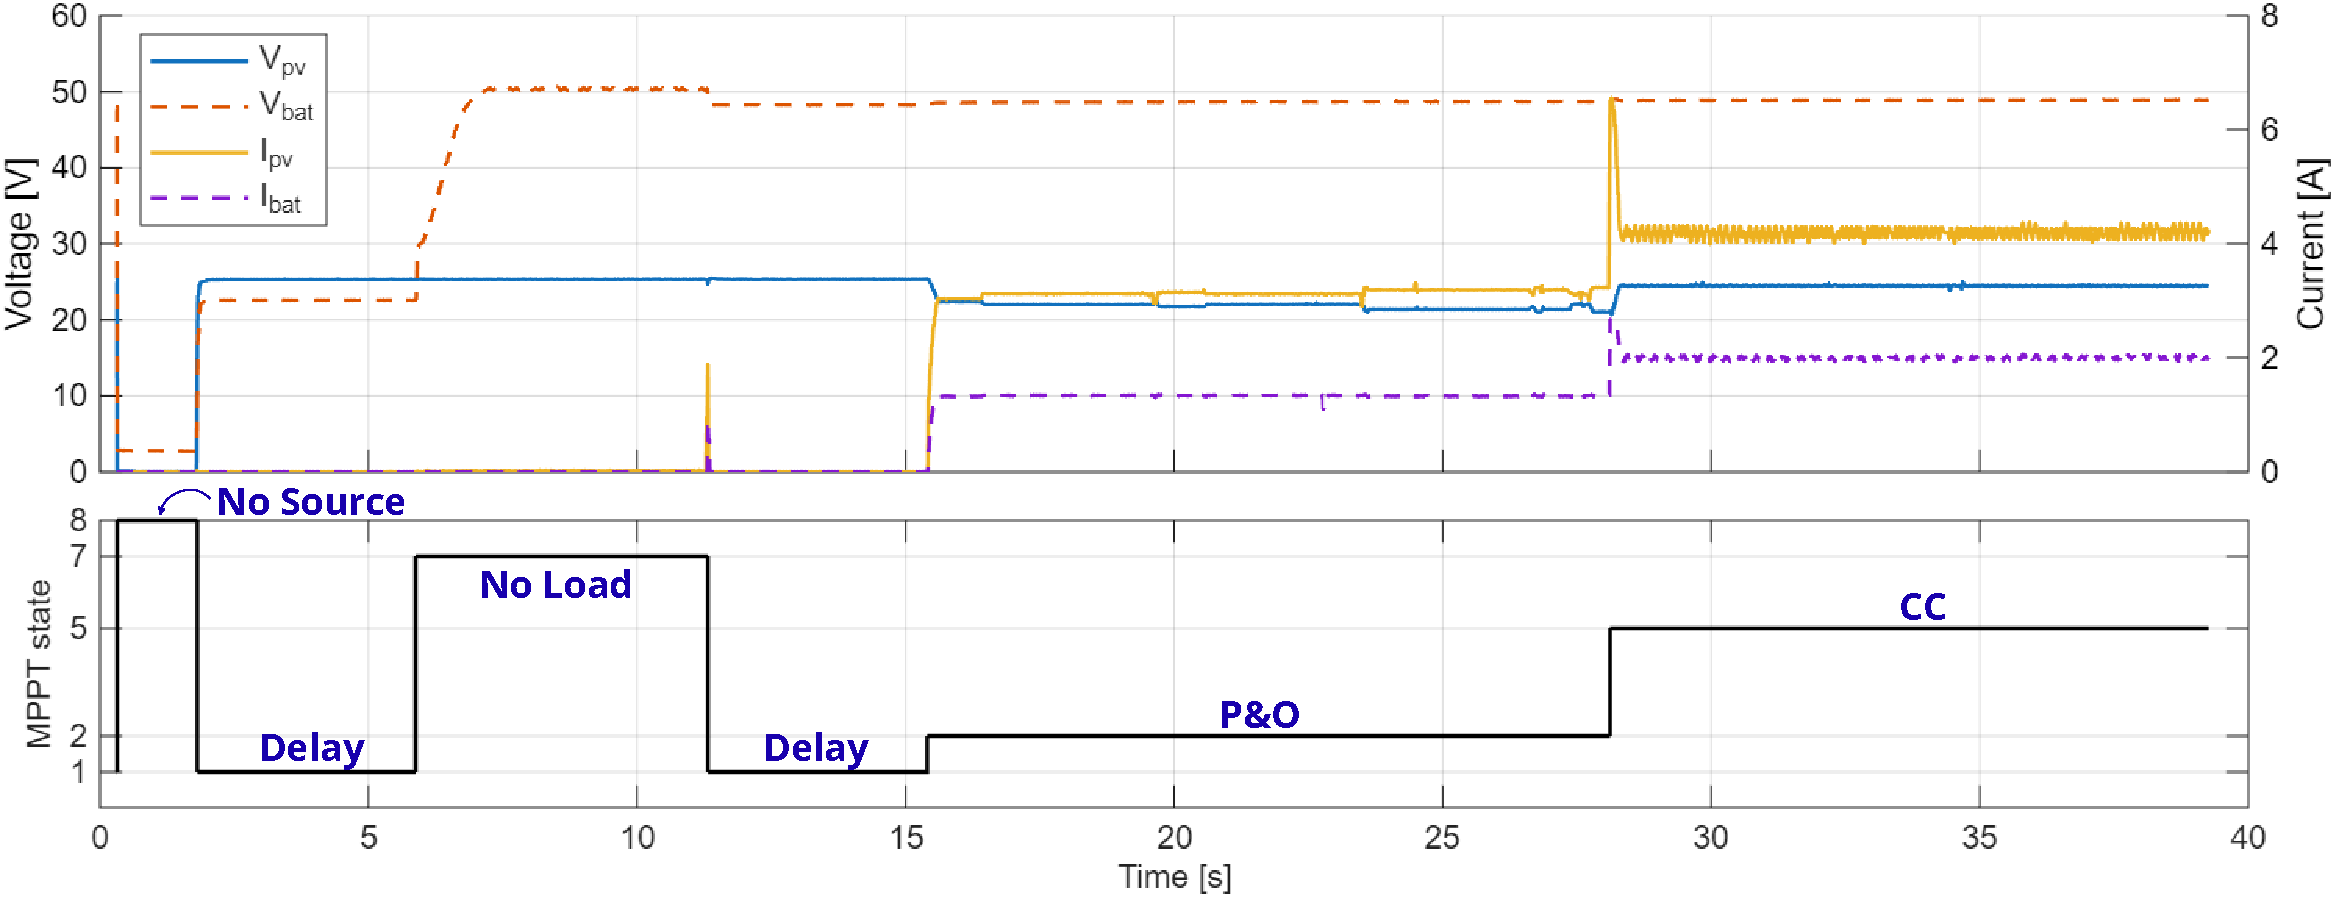
\includegraphics[width=\linewidth]{Images/LAB_res/MPPT states1_1.pdf} 
            \caption{State machine operation over time.} 
            \label{fig:state machine}
        \end{figure} 

    The sweep mode was disabled for this test because its operation with a power supply resulted in occasional overcurrent events. However, when using a real solar panel, the sweep mode operated as expected, as shown in Figure~\ref{fig:state machine2}. At approximately $27~\mathrm{s}$, the sweep was initiated, causing the \ac{pv} voltage to gradually increase while the current decreased. After a few seconds, the sweep was completed, and the operating point transitioned to the \ac{mpp}, while the \ac{peo} was simultaneously initiated. During the sweep, two states were observed: the sweep delay state, which occupied most of the sweep duration, and the sweep state, during which the duty cycle was progressively decreased.


        \begin{figure}[!ht] 
            \centering 
            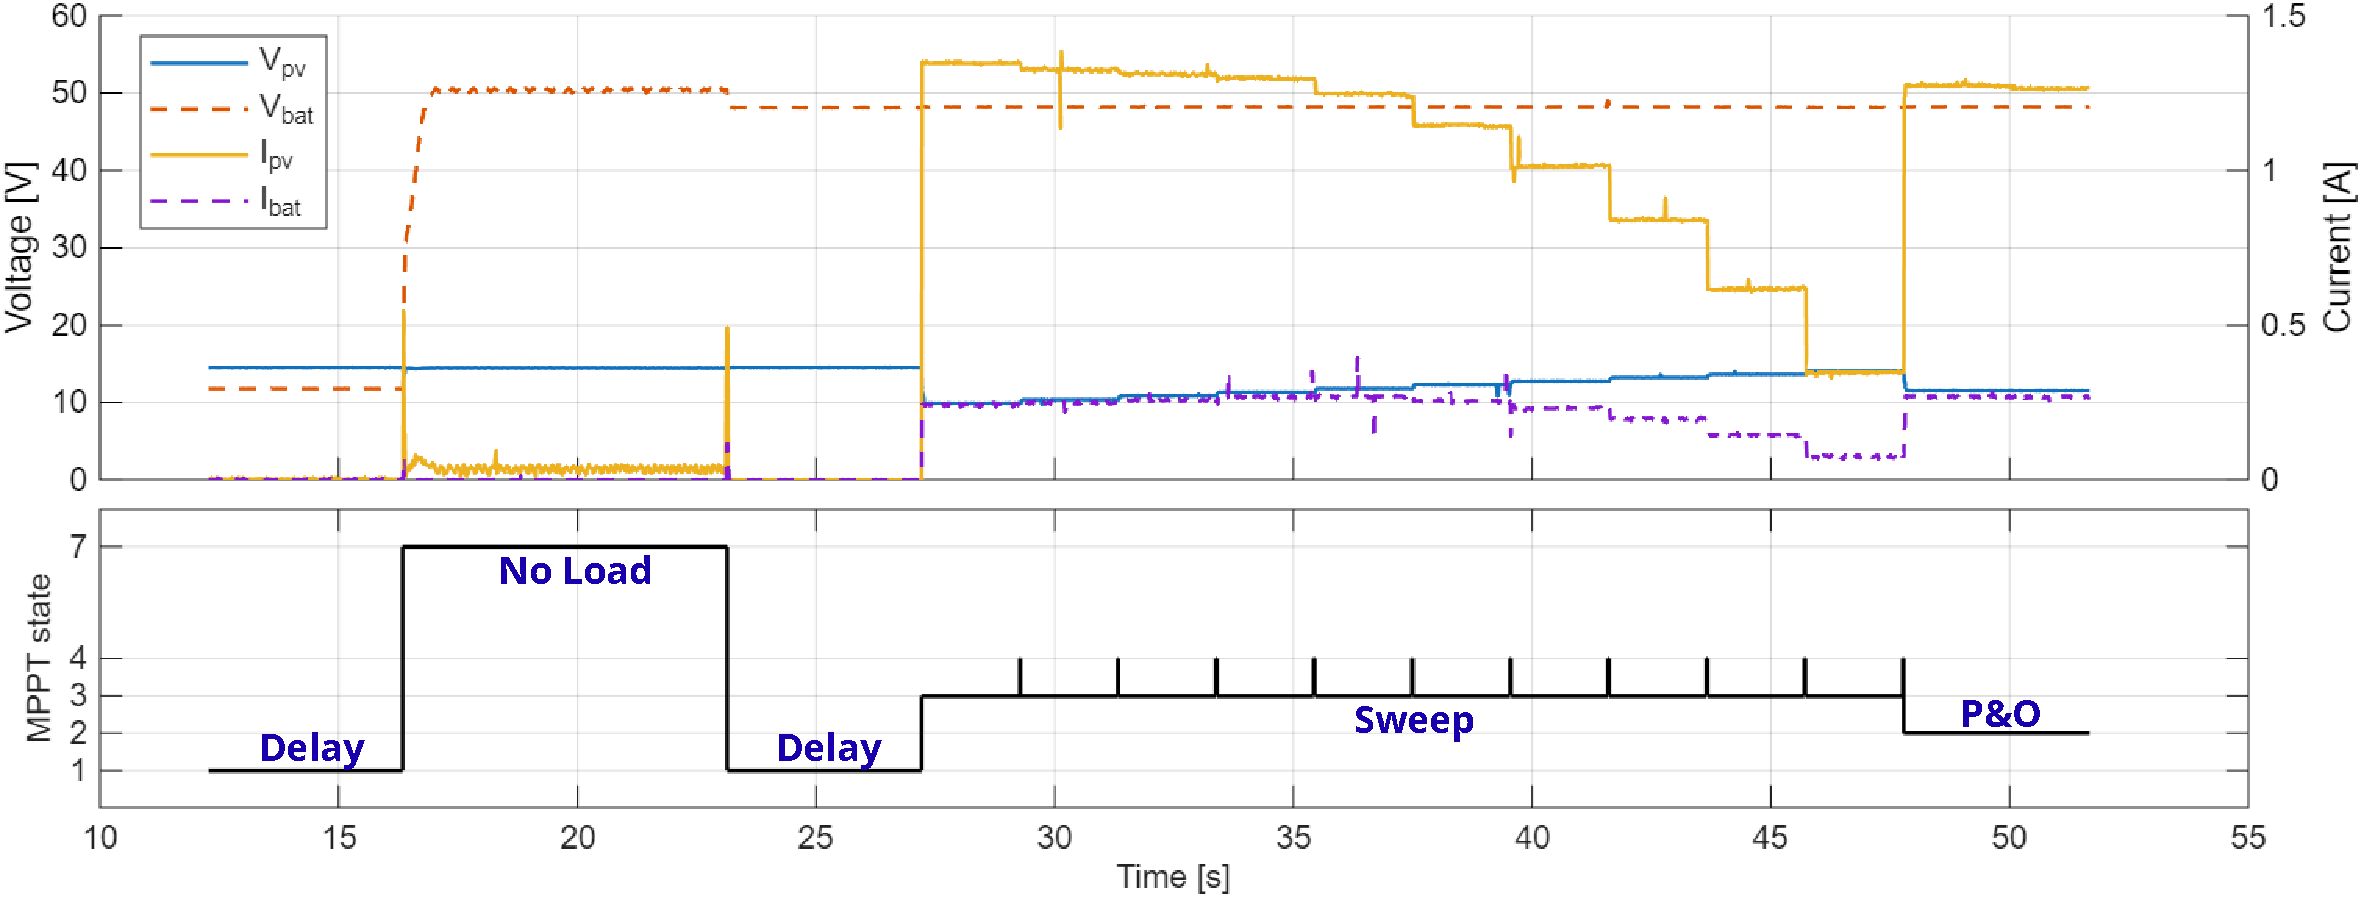
\includegraphics[width=\linewidth]{Images/LAB_res/MPPT states2_1.pdf} 
            \caption{State machine operation over time (sweep mode).} 
            \label{fig:state machine2}
        \end{figure} 


        The \ac{cv} and charge finished states are demonstrated later during a complete charging cycle. 

    \subsection{Efficiency}
        To validate the converter's efficiency under different current and voltage inputs, an irradiance sweep was performed with $10~\mathrm{W/m}^2$ steps from $100~\mathrm{W/m}^2$ to $1000~\mathrm{W/m}^2$. Each irradiance level is maintained for 2~s to ensure that the algorithm is stable. All the values measured during this time are used to compute an average. Additionally, outliers were removed for better results. 

        The result is an efficiency curve (Figure~\ref{fig:eff over current}) that increases with both the input current and the irradiance, which are approximately proportional. Since the test was performed with different solar panel parameters, three curves were obtained. The converter is clearly more efficient at higher input voltages, that is, for panels with more cells in series.

        \begin{figure}[!ht] 
            \centering 
            \begin{minipage}{0.49\textwidth}
                \centering 
                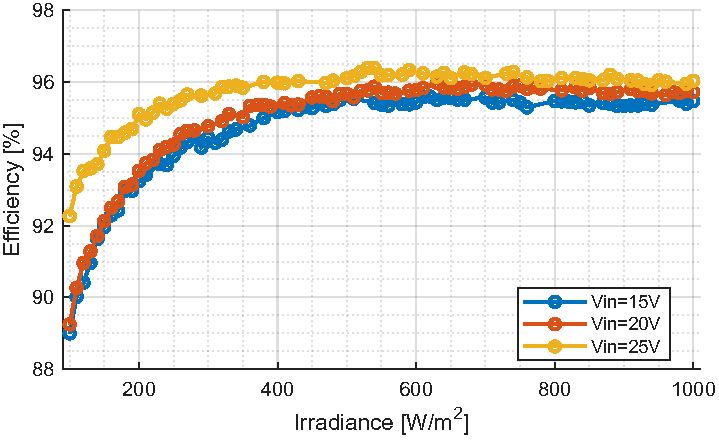
\includegraphics[width=\linewidth]{Images/LAB_res/eff_ipv2.pdf} 
                \caption{Converter efficiency over different input voltages and irradiance ($V_\mathrm{bat} = 43.4~\mathrm{V}$).} 
                \label{fig:eff over current}
            \end{minipage} 
            \hfill 
            \begin{minipage}{0.49\textwidth} 
                \centering 
                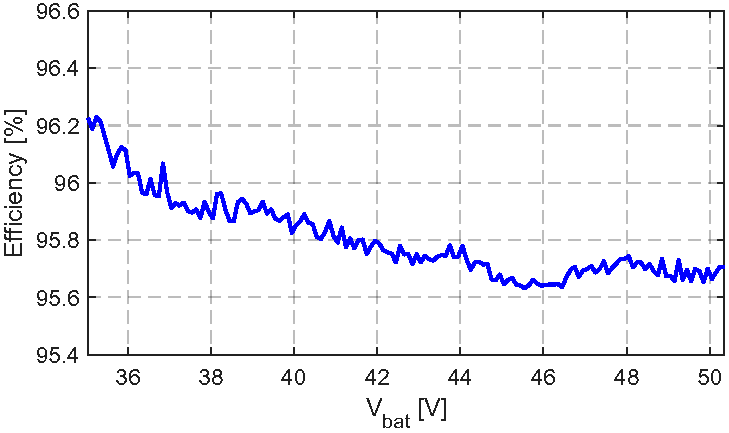
\includegraphics[width=\linewidth]{Images/LAB_res/eff_vout2.pdf} 
                \caption{Converter efficiency over output voltage ($V_\mathrm{pv} = 21.3~\mathrm{V}$ and $I_\mathrm{pv} = 6.5~\mathrm{A}$).} 
                \label{fig:eff over output voltage}
            \end{minipage} 
        \end{figure}


        Both trends are expected. At low currents, the efficiency is lower because the constant losses required to power the electronics (\ac{mcu}, sensors, etc.) have a larger relative impact. As the current increases, those losses become less significant and the efficiency stabilizes. After around 3~A, the converter switching losses become dominant. Since they increase with the input current, a slight downward slope of the curve is expected.

        The higher efficiency at higher input voltage is explained by the fact that a boost converter is more efficient at lower duty cycles. From equation \ref{eq:duty}, for a given output voltage the duty cycle decreases as the input voltage increases. Therefore, increasing the number of cells in series reduces the duty cycle and improves the efficiency.

        On the other hand, if the input voltage is constant and the output voltage increases (Figure~\ref{fig:eff over output voltage}), efficiency decreases for the same reason. Equation \ref{eq:duty} shows that for a fixed input voltage, the duty cycle increases and therefore efficiency decreases.   


    \subsection{Tracking speed}
        Several configurations were tested to optimize the \ac{peo} algorithm. Following the tuning process, the final configuration was defined as shown in Table~\ref{tab:MPPT_config}.

        \begin{table}[!ht]
        \centering
        \caption{MPPT parameters.}
        \label{tab:MPPT_config}
            \begin{tabular}{|c|c|c|c|}
            \hline
            Sampling frequency & MPPT frequency & Step size & Power Dead Band \\
            \hline
            1~kHz & 50~Hz & 0.7~\% & 700~mW \\
            \hline
            \end{tabular}
        \end{table}

        To evaluate the performance of the \ac{mppt} algorithm under varying environmental conditions, several Python scripts were developed to control the temperature and irradiance of the power source. Through a LAN connection, the scripts transmit TCP messages to the power supply, allowing its environmental parameters to be modified during the tests.

        Two test scenarios were defined:

        \begin{enumerate}[leftmargin=4em, itemsep=1pt, topsep=2pt]
            \item \textbf{Irradiance staircase:} The test starts at an irradiance of $1000~\mathrm{W/m}^2$, which is subsequently reduced by $200~\mathrm{W/m}^2$ at approximately 2~s intervals until reaching $200~\mathrm{W/m}^2$. The irradiance is then increased to $1000~\mathrm{W/m}^2$ in one step.

            \item \textbf{Temperature staircase:} The test starts at $25~^\circ\mathrm{C}$, after which the temperature is increased in $10~^\circ\mathrm{C}$ steps at 2~s intervals until reaching $85~^\circ\mathrm{C}$. The temperature is then decreased to $25~^\circ\mathrm{C}$ in one step.
        \end{enumerate}

        Both tests were divided into two phases. In the first phase, the environmental parameters were varied gradually to evaluate the tracking performance under normal operating conditions. In the second phase, more abrupt changes were introduced to assess the tracking performance under more demanding conditions. This approach allows the response of the algorithm to be evaluated for both gradual and rapid variations in the operating conditions.

        The results of the irradiance and temperature staircase tests are presented in Figures~\ref{fig:irr_stairway} and \ref{fig:temp_stairway}, respectively. Overall, the algorithm demonstrated satisfactory tracking performance, maintaining the operating point close to the \ac{mpp} while responding to changes in the environmental conditions.


        \begin{figure}[!ht]
            \centering
            \begin{minipage}[b]{0.49\textwidth}
                \centering
                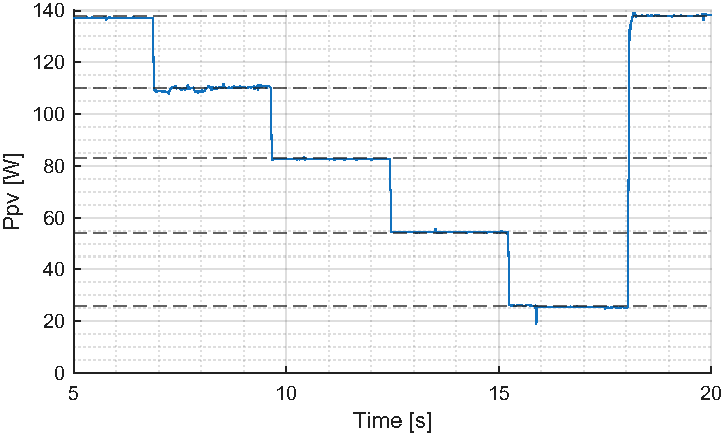
\includegraphics[width=\textwidth]{Images/LAB_res/irr_stairway.pdf}
                \caption{Power response for the "Irradiance stairway" test.}
                \label{fig:irr_stairway}
            \end{minipage}
            \hfill
            \begin{minipage}[b]{0.49\textwidth}
                \centering
                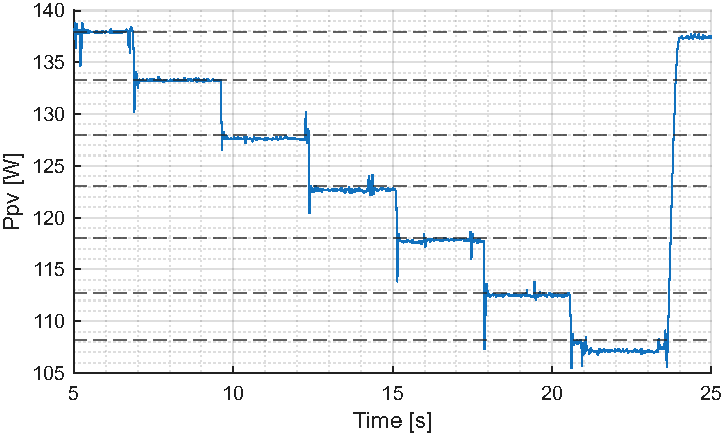
\includegraphics[width=\textwidth]{Images/LAB_res/temp_stairway.pdf}
                \caption{Power response for the "Temperature stairway" test.}
                \label{fig:temp_stairway}
            \end{minipage}
        \end{figure}

        For both tests, the measured tracking time, defined as the time required to reach within $\pm 5\%$ of the \ac{mpp}, was typically below 100~ms, based on the measurements obtained during the first phase. When the irradiance was increased from $200~\mathrm{W/m}^2$ to $1000~\mathrm{W/m}^2$, the tracking time was slightly higher but remained below 100~ms. The highest measured tracking time occurred when the solar panels were cooled from $85~^\circ\mathrm{C}$ to $25~^\circ\mathrm{C}$, for which a tracking time of approximately 200~ms was measured. Individual tracking times for each test condition are not presented, as the response was nearly instantaneous in most cases, making accurate measurement difficult with the available instrumentation.

        In addition to the tracking speed, the \ac{mppt} algorithm demonstrated a high tracking accuracy, with an average value of approximately 99\%. Nevertheless, some deviations from the \ac{mpp} were observed under specific operating conditions, particularly at $85~^\circ\mathrm{C}$. These deviations are likely related to measurement noise, although this could not be conclusively verified.

        
    
\section{Charging test}
    To prove the functionality of the developed prototype, two charging tests were recorded. Both tests use the smaller battery described in section~\ref{sec:battery}.

    By using the SM 1500-CP-30 power supply in photovoltaic function connected to the \ac{mppt} charger, the battery was fully charged. Figure~\ref{fig:full charge in lab} shows the result where the CC-CV charging curve was achieved. In \ac{cc} mode, the algorithm tracked the \ac{mpp} successfully. At \ac{cv}, the output voltage is constant, and the output current dropped slowly. 

    \begin{figure}[!ht] 
        \centering 
        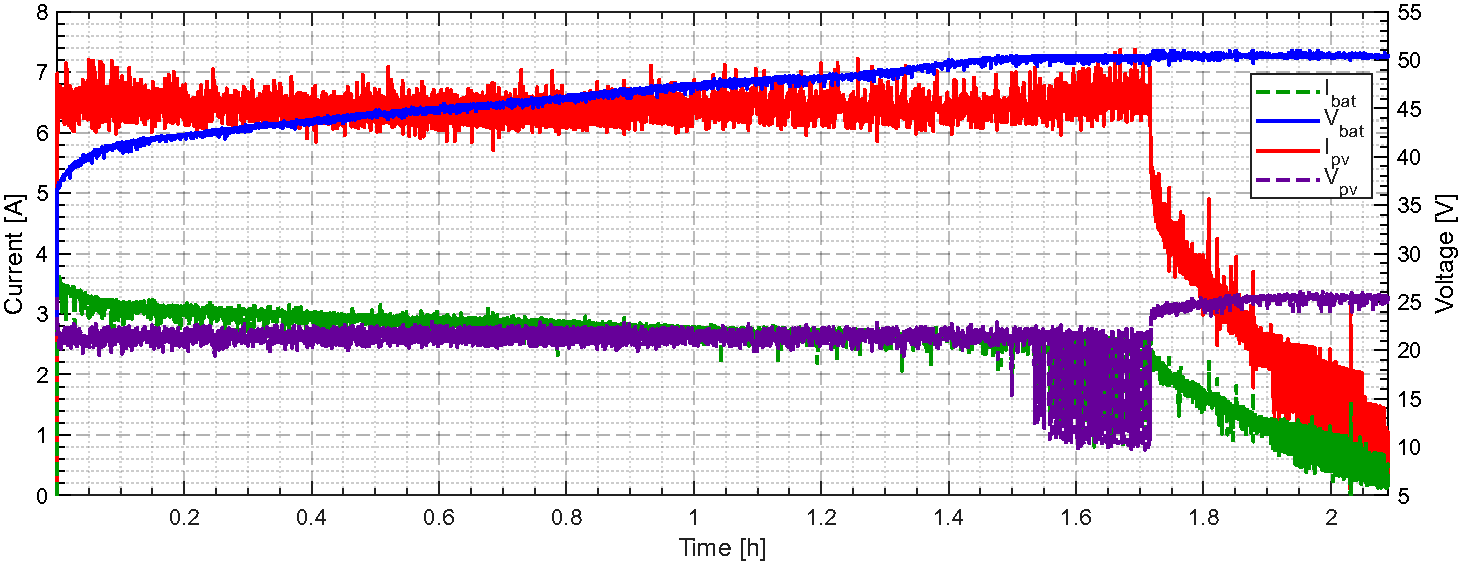
\includegraphics[width=0.8\linewidth]{Images/LAB_res/charging_test_lab.pdf} 
        \caption{Full battery charge in laboratory.} 
        \label{fig:full charge in lab}
    \end{figure} 

    The last test is a field test (on shore) with a solar panel. Several attempts were made to perfect the performance of the prototype. A lot of errors were encountered and fixed. For example, the first time the test was performed, it was used a solar panel of only 20 cells, which was never tested before, and did not work correctly because the duty cycle upper limit was too low. By increasing the duty cycle upper limit, the issue was resolved. Then in prototype version 1.2, the noise was reduced and the power deadband was too high, which made the \ac{mppt} algorithm not able to track slow environment changes. After some tests, the power deadband was completely removed. Some other adjustments were made to the state machine and the final test was performed.

    The final test was performed with two solar panels in series, with a total of 38 cells. The test was performed in a cloudy day, with a lot of irradiance variations. The results show the correct operation of the \ac{cc}-\ac{cv} charging curve, and the correct operation of the \ac{mppt} algorithm, Figure~\ref{fig:full charge in field}.

    Since the test was performed in a cloudy day, the irradiance was very unstable, which induces \acs{pv} current variations. The temperature of the solar panel was stable and therefore the \ac{pv} voltage only adjust slightly to reach the \ac{mpp}. 

    The test was interrupted one time due to an accidental disconnection of the solar panel.
    
    
    \begin{figure}[!ht] 
        \centering 
        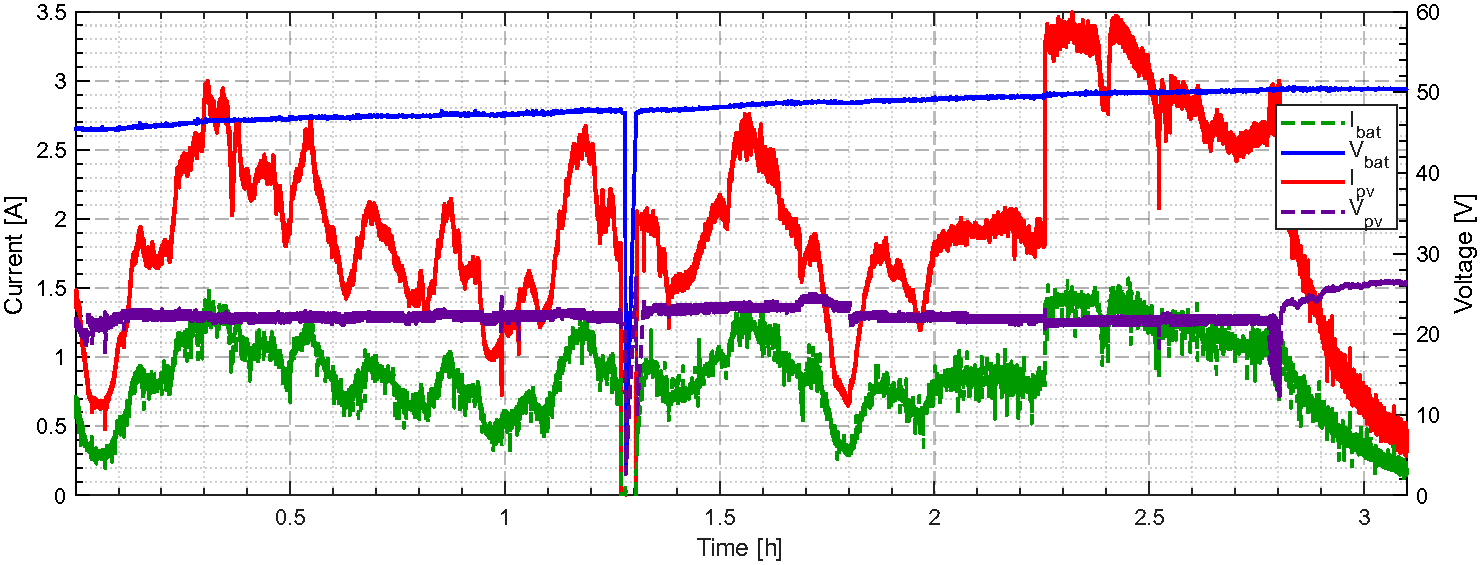
\includegraphics[width=0.8\linewidth]{Images/LAB_res/charging_test4.pdf} 
        \caption{Battery charging test. Voltage and current curve.} 
        \label{fig:full charge in field}
    \end{figure} 


    % \textcolor{red}{Add tests in water if time permits.}